% Created 2014-11-12 Wed 20:44
\documentclass[presentation]{beamer}
\usepackage[utf8]{inputenc}
\usepackage[T1]{fontenc}
\usepackage{fixltx2e}
\usepackage{graphicx}
\usepackage{longtable}
\usepackage{float}
\usepackage{wrapfig}
\usepackage{rotating}
\usepackage[normalem]{ulem}
\usepackage{amsmath}
\usepackage{textcomp}
\usepackage{marvosym}
\usepackage{wasysym}
\usepackage{amssymb}
\usepackage{hyperref}
\tolerance=1000
\usetheme{codemotion-madrid2014}
\author{}
\date{2014-11-22}
\title{}
\hypersetup{
  pdfkeywords={continuous-delivery, maven, jenkins, docker, puppet, shipyard, mcollective},
  pdfsubject={Continuous Delivery with Maven, Jenkins, Docker, Puppet, Shipyard and MCollective},
  pdfcreator={Emacs 24.3.1 (Org mode 8.2.6)}}
\begin{document}

\title[Continuous Delivery]{}
\author[Jose San Leandro]{}
\addtobeamertemplate{block begin}{\pgfsetfillopacity{0.5}}{\pgfsetfillopacity{1}}
\addtobeamertemplate{block alerted begin}{\pgfsetfillopacity{0.5}}{\pgfsetfillopacity{1}}
\addtobeamertemplate{block example begin}{\pgfsetfillopacity{0.5}}{\pgfsetfillopacity{1}}
\section{}
\label{sec-1}
{
\setbeamertemplate{navigation symbols}{}
\begin{frame}[label=sec-1-1]{}
\begin{tikzpicture}[remember picture,overlay]
\node[at=(current page.center)] {
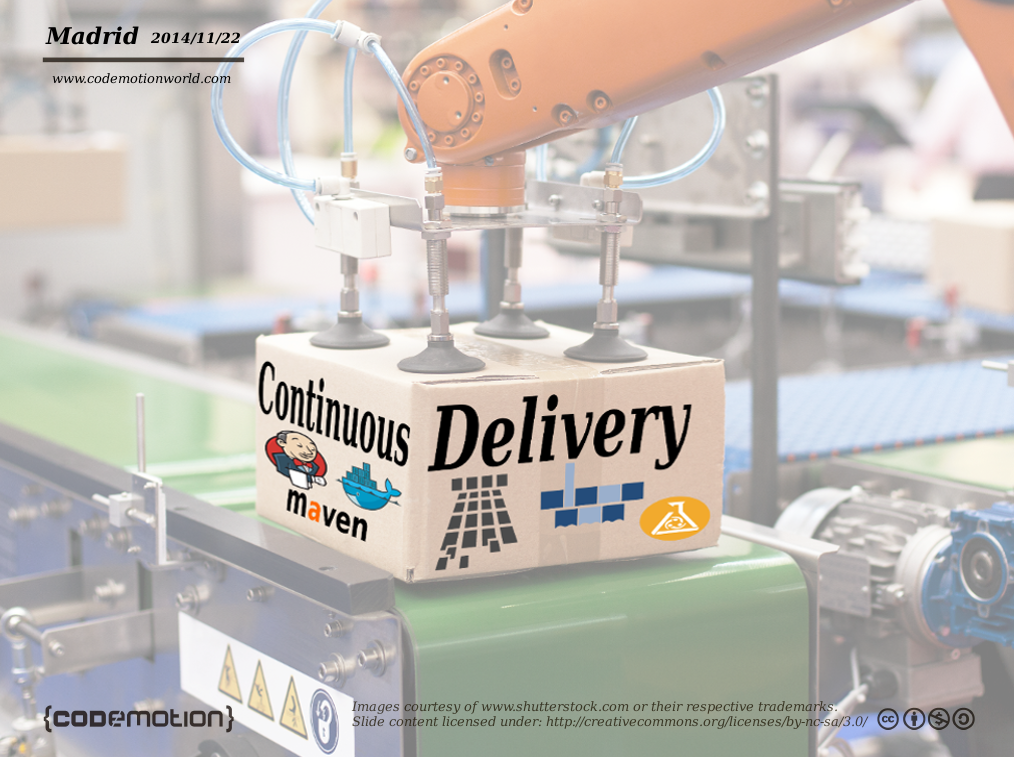
\includegraphics[width=\paperwidth]{frontpage.png}
};
\node[shift={(4.5cm, -0.44cm)}, right] at (current page.north west) {};
\end{tikzpicture}

\end{frame}
} % background

\section{Introduction}
\label{sec-2}

{
\setbeamertemplate{navigation symbols}{}
\begin{frame}[label=sec-2-1]{}
\begin{tikzpicture}[remember picture,overlay]
\node[at=(current page.center)] {

\includegraphics[width=\paperwidth]{what-is-this-all-about-bg.png}
};
\node[shift={(4.5cm, -0.44cm)}, right] at (current page.north west) {};
\end{tikzpicture}

\begin{block}{What is this all about?}

\begin{itemize}
\item A brief introduction to Continuous Delivery.
\item How each tool fits in the big picture.
\item The approach I propose, without the pain.
\item Help to get you started on your own.
\item Advance towards Continuous Deployment.
\end{itemize}
\end{block}
\end{frame}
} % background

\section{Continuous Delivery}
\label{sec-3}
{
\setbeamertemplate{navigation symbols}{}
\begin{frame}[label=sec-3-1]{}
\begin{tikzpicture}[remember picture,overlay]
\node[at=(current page.center)] {
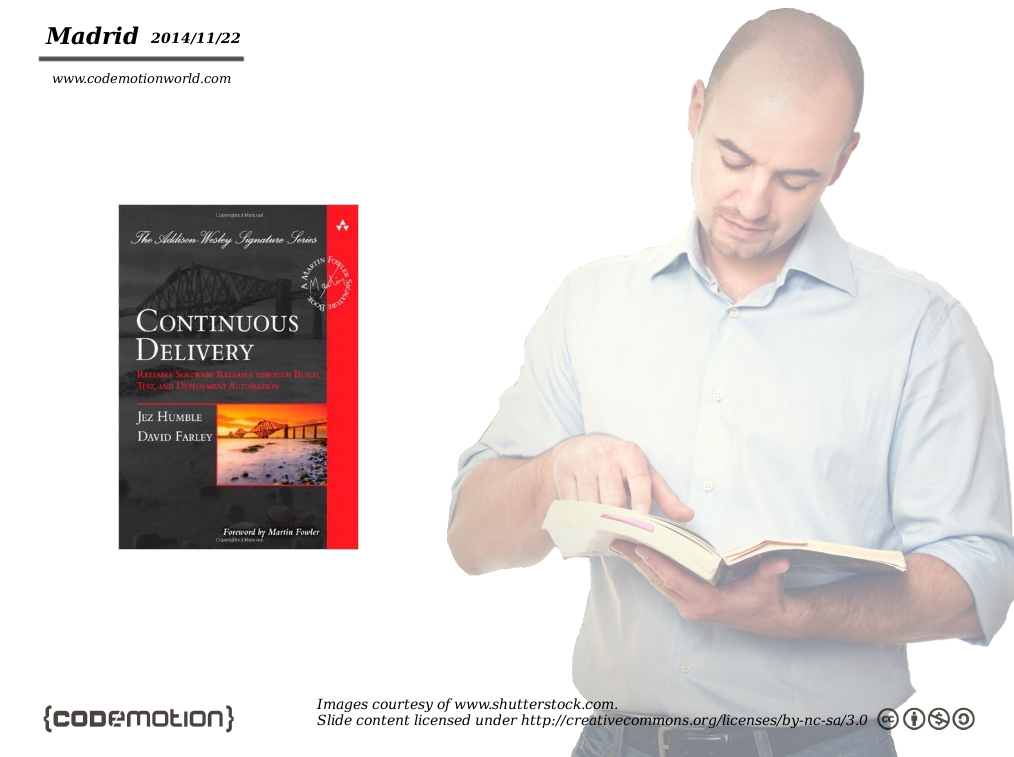
\includegraphics[width=\paperwidth]{cd-book-bg.png}
};
\node[shift={(4.5cm, -0.44cm)}, right] at (current page.north west) {};
\end{tikzpicture}

\begin{columns}
\begin{column}{0.4\textwidth}

\end{column}

\begin{column}{0.6\textwidth}
\begin{quotation} %% Continuous Delivery - Jez Humble and David Farley

\textit{``Encouraging greater collaboration between everyone involved in software delivery in order to release valuable software faster and more reliably.''}
\end{quotation}
\end{column}
\end{columns}
\end{frame}
} % background

{
\setbeamertemplate{navigation symbols}{}
\begin{frame}[label=sec-3-2]{}
\begin{tikzpicture}[remember picture,overlay]
\node[at=(current page.center)] {
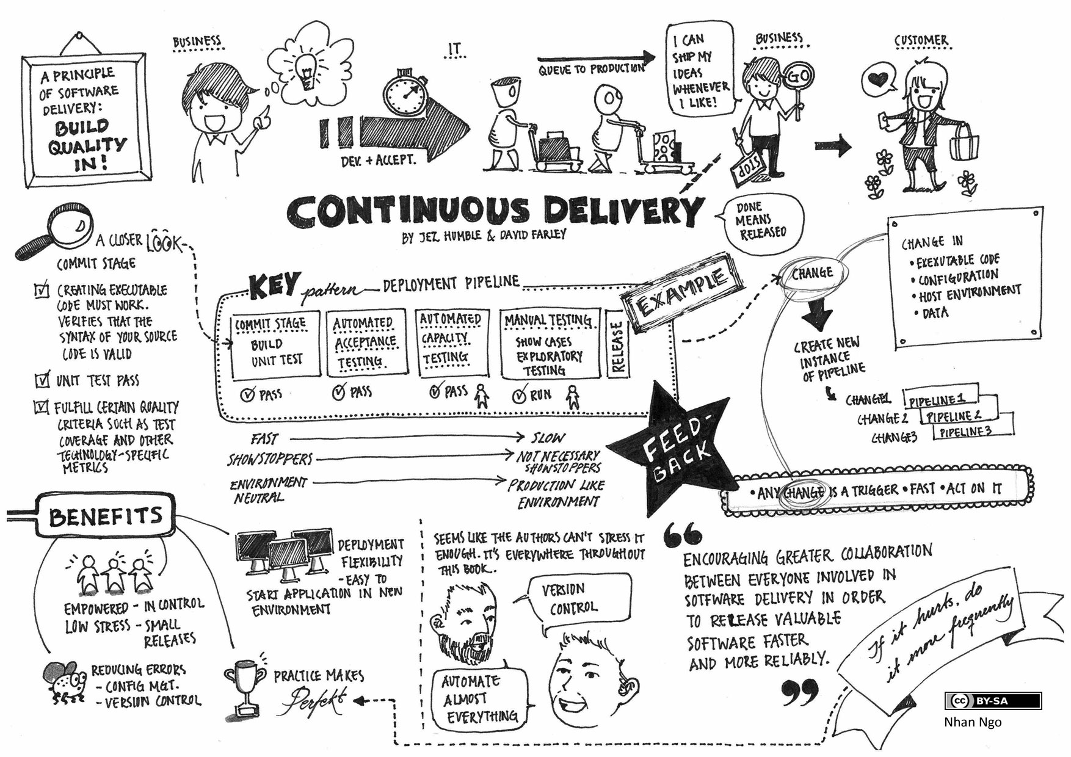
\includegraphics[width=\paperwidth]{continuous-delivery-pipeline-bg.png}
};
\node[shift={(4.5cm, -0.44cm)}, right] at (current page.north west) {};
\end{tikzpicture}

\end{frame}
} % background


{
\setbeamertemplate{navigation symbols}{}
\begin{frame}[label=sec-3-3]{Automation}
\begin{tikzpicture}[remember picture,overlay]
\node[at=(current page.center)] {
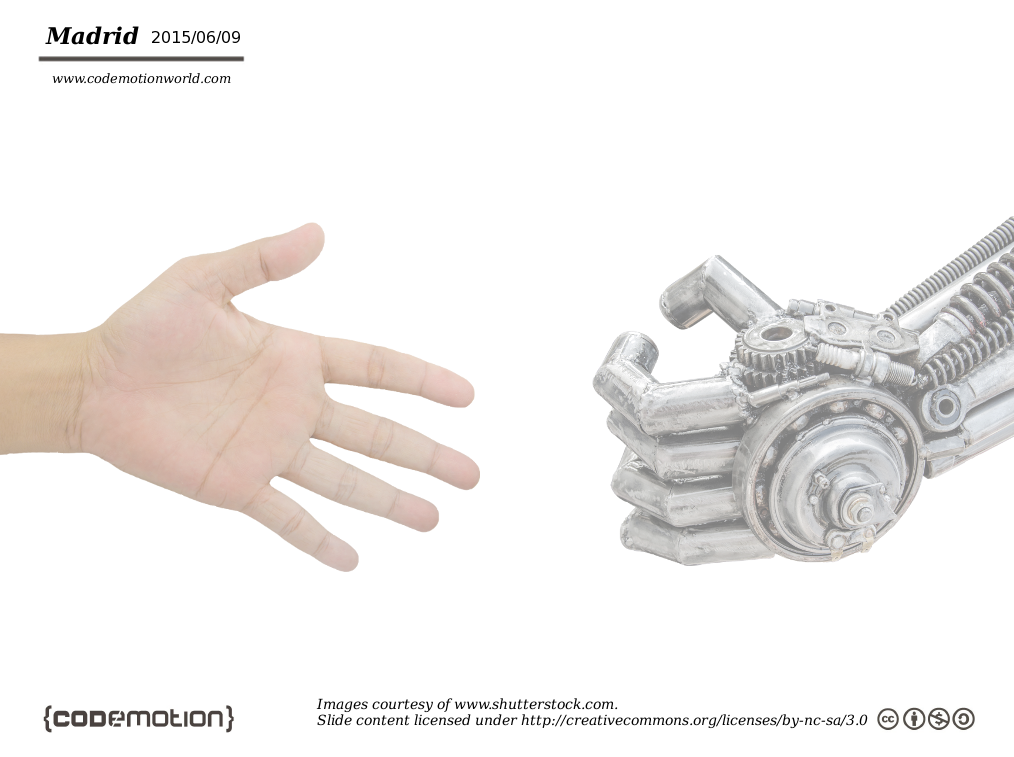
\includegraphics[width=\paperwidth]{cd-automation-bg.png}
};
\node[shift={(4.5cm, -0.44cm)}, right] at (current page.north west) {Automation};
\end{tikzpicture}

\begin{block}{Bots welcome}

\begin{itemize}
\item Speed up the release of new features.
\item Special focus on risk: automate everything!
\item Advance towards Continuous Deployment.
\item No need for code freeze.
\item Automated tagging.
\end{itemize}
\end{block}
\end{frame}
} % background

\section{What is this all about?}
\label{sec-4}

\section{Maven}
\label{sec-5}

{
\setbeamertemplate{navigation symbols}{}
\begin{frame}[label=sec-5-1]{}
\begin{tikzpicture}[remember picture,overlay]
\node[at=(current page.center)] {
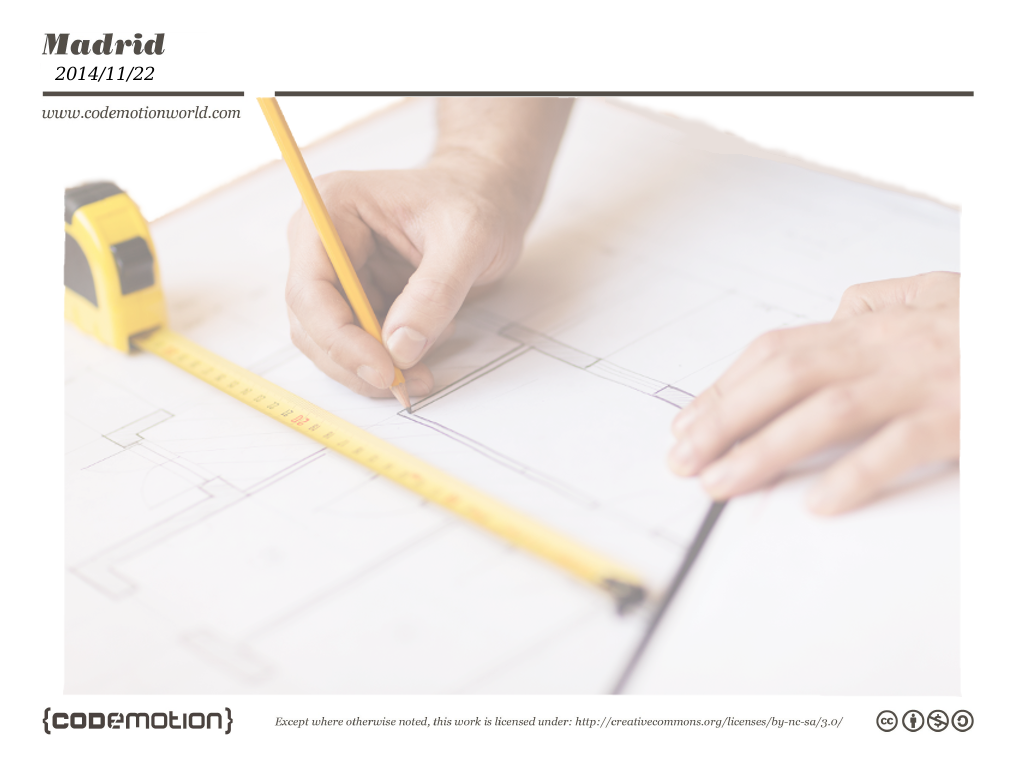
\includegraphics[width=\paperwidth]{maven-definition-bg.png}
};
\node[shift={(4.5cm, -0.44cm)}, right] at (current page.north west) {};
\end{tikzpicture}

\begin{columns}
\begin{column}{0.6\textwidth}
\begin{quotation} %% Maven quote

\textit{``Apache Maven is a software project management and comprehension tool. Based on the concept of a project object model (POM), Maven can manage a project's build, reporting and documentation from a central piece of information.''}
\end{quotation}
\end{column}

\begin{column}{0.4\textwidth}

\includegraphics[width=100]{maven.png}

\small{http://apache.maven.org}
\end{column}
\end{columns}
\end{frame}
} % background

{
\setbeamertemplate{navigation symbols}{}
\begin{frame}[label=sec-5-2]{Modularization}
\begin{tikzpicture}[remember picture,overlay]
\node[at=(current page.center)] {
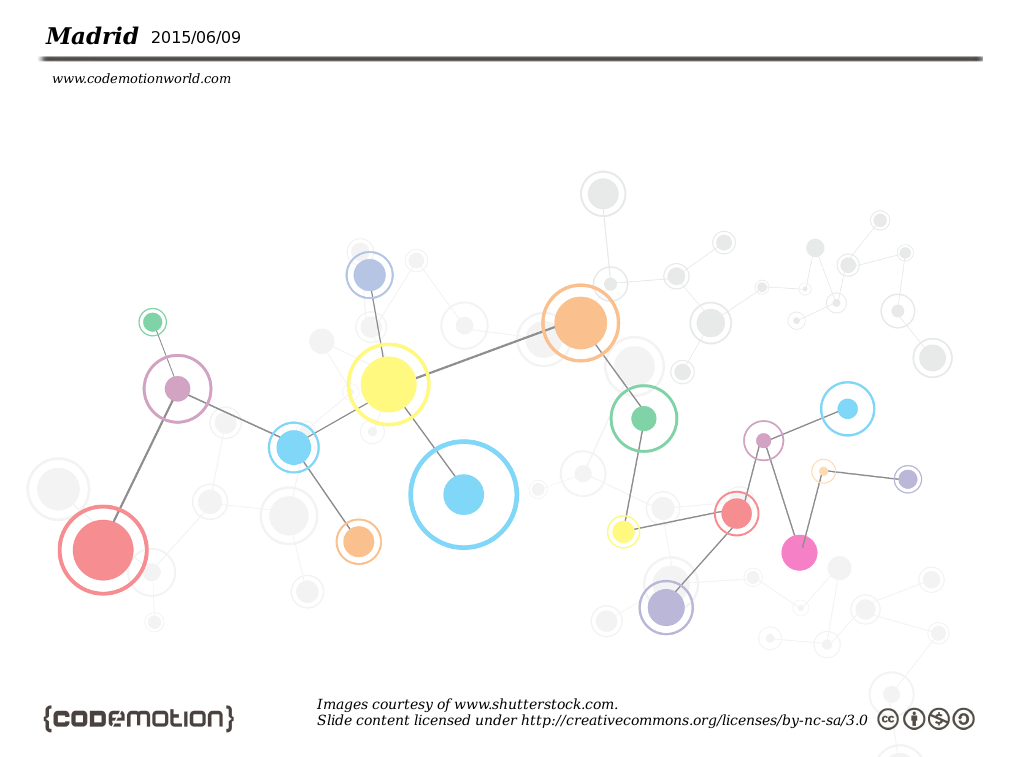
\includegraphics[width=\paperwidth]{maven-graph-bg.png}
};
\node[shift={(4.5cm, -0.44cm)}, right] at (current page.north west) {Modularization};
\end{tikzpicture}

\begin{block}{Convention}
\begin{itemize}
\item All logic is isolated in its own module.
\item No multi-module projects, unless for WARs.
\item All modules inherit from a common, logic-less module: the parent POM.
\end{itemize}
\end{block}
\end{frame}
} % background

{
\setbeamertemplate{navigation symbols}{}
\begin{frame}[label=sec-5-3]{Parent POM}
\begin{tikzpicture}[remember picture,overlay]
\node[at=(current page.center)] {
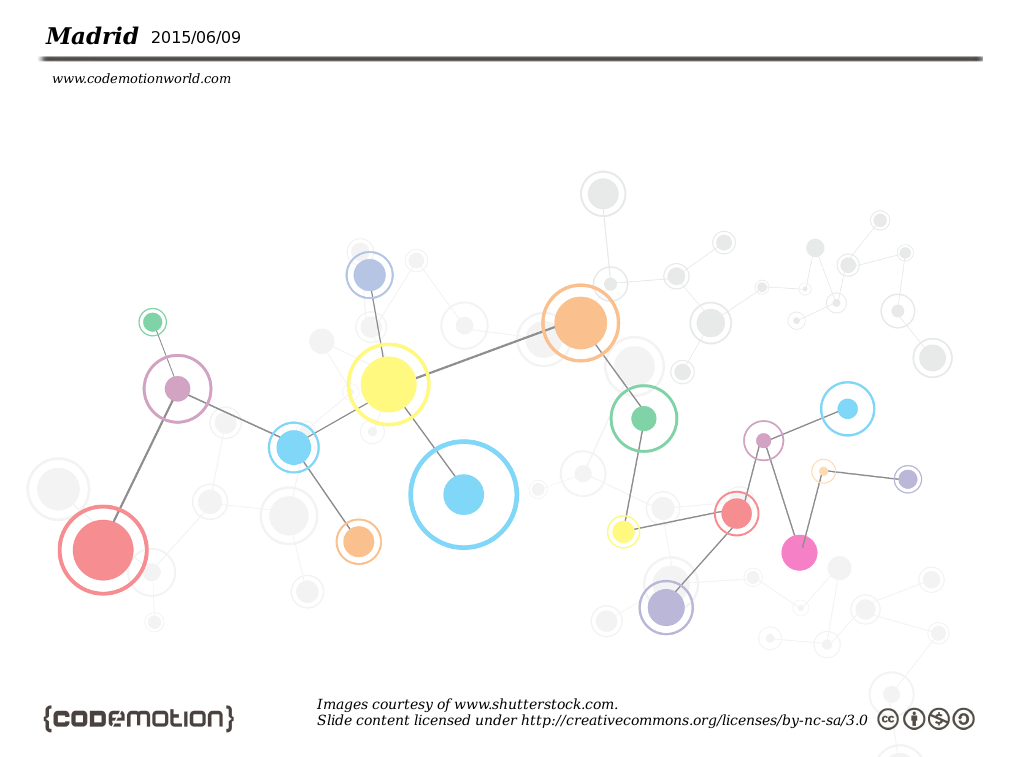
\includegraphics[width=\paperwidth]{maven-graph-bg.png}
};
\node[shift={(4.5cm, -0.44cm)}, right] at (current page.north west) {Parent POM};
\end{tikzpicture}

\begin{block}{According to Maven, a parent\ldots{}}

\begin{itemize}
\item Declares all dependencies in one place.
\item Ensures all modules use the same versions of the dependencies.
\item Defines common configurations for maven plugins.
\item Simplifies child poms.
\item Uses Maven properties to specify the versions of in-house modules.
\end{itemize}
\end{block}
\end{frame}
} % background


{
\setbeamertemplate{navigation symbols}{}
\begin{frame}[label=sec-5-4]{Versioning}
\begin{tikzpicture}[remember picture,overlay]
\node[at=(current page.center)] {
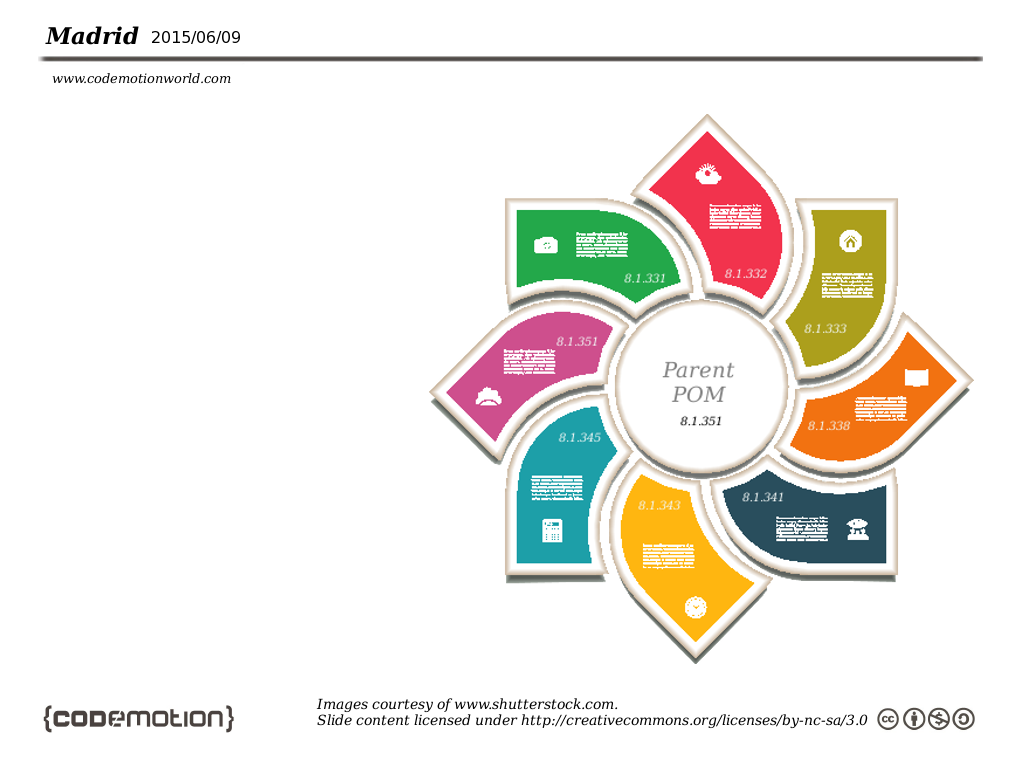
\includegraphics[width=\paperwidth]{maven-versioning-bg.png}
};
\node[shift={(4.5cm, -0.44cm)}, right] at (current page.north west) {Versioning};
\end{tikzpicture}

\begin{columns}
\begin{column}{0.5\textwidth}
\begin{block}{Versions are unique and time-ordered}

\begin{itemize}
\item All in-house modules, share the same version: \texttt{latest-SNAPSHOT}.
\item All local environments get always up-to-date code.
\item Versions are resolved when generating releases.
\end{itemize}
\end{block}
\end{column}

\begin{column}{0.5\textwidth}

\end{column}
\end{columns}
\end{frame}
} % background

\section{Jenkins}
\label{sec-6}

{
\setbeamertemplate{navigation symbols}{}
\begin{frame}[label=sec-6-1]{}
\begin{tikzpicture}[remember picture,overlay]
\node[at=(current page.center)] {
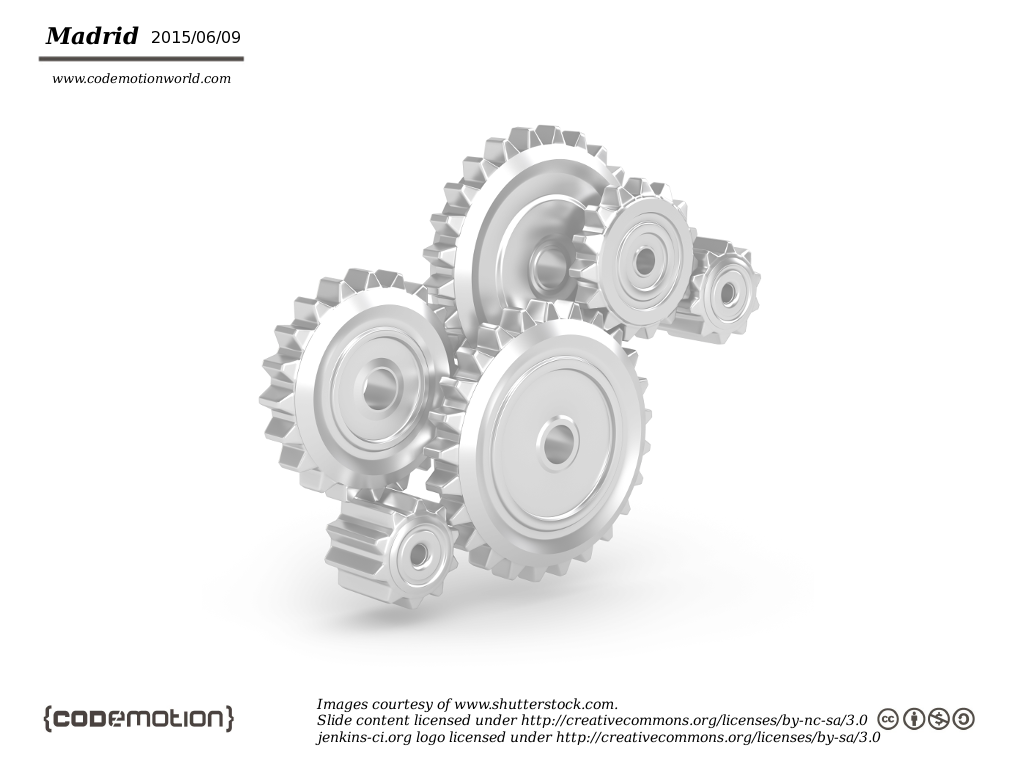
\includegraphics[width=\paperwidth]{jenkins-definition-bg.png}
};
\node[shift={(4.5cm, -0.44cm)}, right] at (current page.north west) {};
\end{tikzpicture}

\begin{columns}
\begin{column}{0.6\textwidth}
\begin{quotation} %% Jenkins

\textit{``An extendable open source continuous integration server.''}
\end{quotation}
\end{column}

\begin{column}{0.4\textwidth}

\includegraphics[width=100]{jenkins.png}

\url{http://jenkins-ci.org}
\end{column}
\end{columns}
\end{frame}
} % background

{
\setbeamertemplate{navigation symbols}{}
\begin{frame}[label=sec-6-2]{\textit{get-new-version} job}
\begin{tikzpicture}[remember picture,overlay]
\node[at=(current page.center)] {
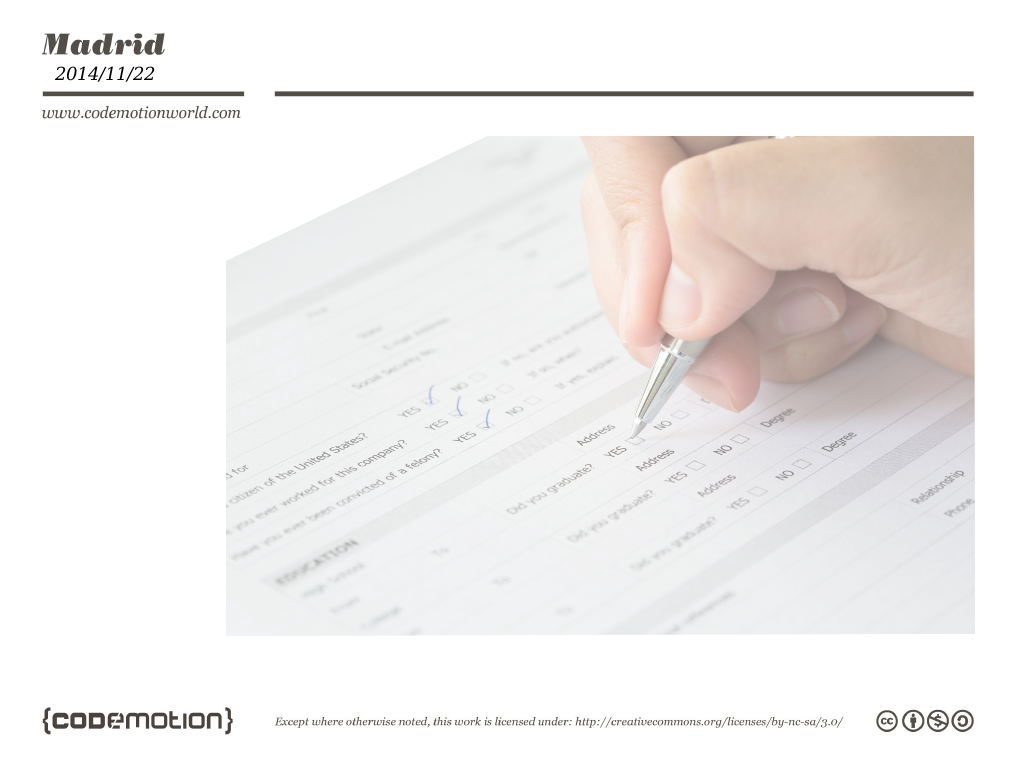
\includegraphics[width=\paperwidth]{jenkins-get-new-version-1-bg.png}
};
\node[shift={(4.5cm, -0.44cm)}, right] at (current page.north west) {\textit{get-new-version} job};
\end{tikzpicture}

\begin{block}{Generates unique version numbers}

\begin{itemize}
\item Helper job to automate the tagging and packaging process.
\item Checks out parent-pom code.
\item Parameterized job with a single parameter: the name of the module triggering the release.
\item Should have higher priority to avoid slot starvation and deadlocks in Jenkins.
\item Expects parent-pom to contain two properties: version.major and version.minor.
\end{itemize}
\end{block}
\end{frame}
} % background

{
\setbeamertemplate{navigation symbols}{}
\begin{frame}[label=sec-6-3]{}
\begin{tikzpicture}[remember picture,overlay]
\node[at=(current page.center)] {

\includegraphics[width=\paperwidth]{jenkins-get-new-version-1b-bg.png}
};
\node[shift={(4.5cm, -0.44cm)}, right] at (current page.north west) {};
\end{tikzpicture}

\begin{columns}
\begin{column}{0.6\textwidth}
\begin{quotation} %% 

\end{quotation}
\end{column}
\end{columns}
\end{frame}
} % background

{
\setbeamertemplate{navigation symbols}{}
\begin{frame}[label=sec-6-4]{\textit{get-new-version} job (2)}
\begin{tikzpicture}[remember picture,overlay]
\node[at=(current page.center)] {
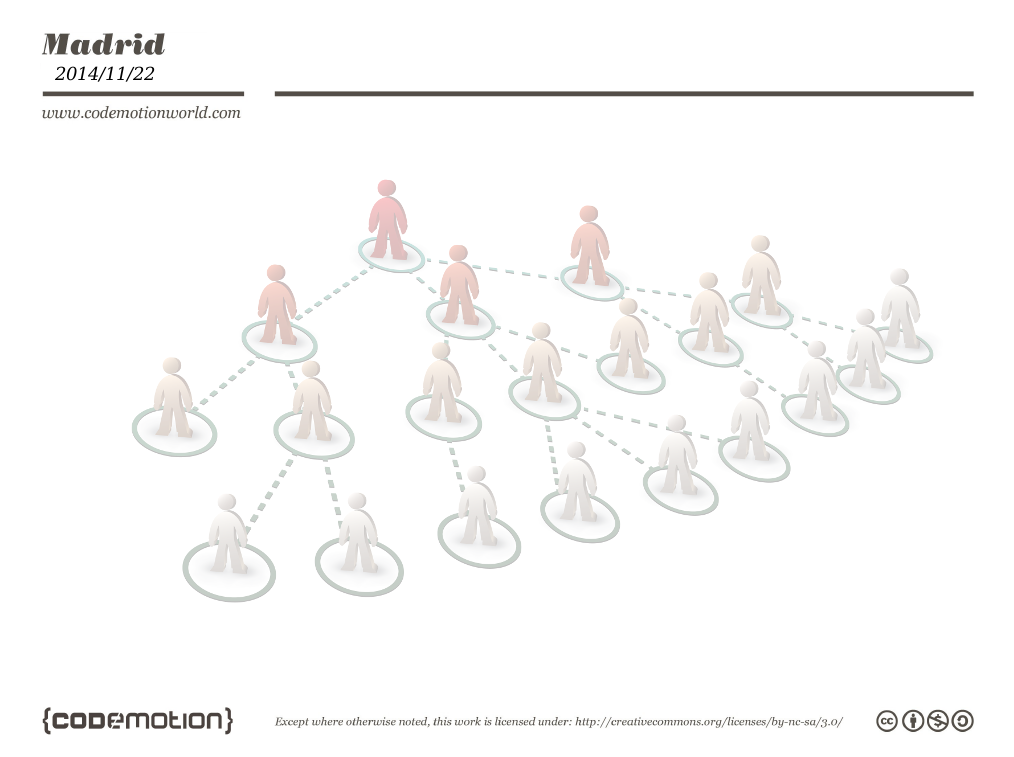
\includegraphics[width=\paperwidth]{jenkins-get-new-version-2-bg.png}
};
\node[shift={(4.5cm, -0.44cm)}, right] at (current page.north west) {\textit{get-new-version} job (2)};
\end{tikzpicture}

\begin{block}{One \textbf{job} to rule them all}

\begin{itemize}
\item When a commit is pushed to the remote repository, Jenkins launches the associated job.
\item The job is a Maven job, which runs \texttt{mvn deploy}.
\item If it succeeds, calls \texttt{get-new-version} with its own name as parameter.
\end{itemize}
\end{block}
\end{frame}
} % background

{
\setbeamertemplate{navigation symbols}{}
\begin{frame}[label=sec-6-5]{\textit{get-new-version} job (3)}
\begin{tikzpicture}[remember picture,overlay]
\node[at=(current page.center)] {

\includegraphics[width=\paperwidth]{jenkins-get-new-version-3-bg.png}
};
\node[shift={(4.5cm, -0.44cm)}, right] at (current page.north west) {\textit{get-new-version} job (3)};
\end{tikzpicture}

\begin{block}{maven-versions-plugin magic}

\begin{itemize}
\item Parses the parent pom and defines a new version using a convention: $V = major.minor.BUILD\_NUMBER$ (provided by Jenkins).
\item Using \textbf{maven-versions-plugin}:
\begin{itemize}
\item Points itself to new version $V$.
\item Uses the latest released versions for all modules.
\item Ensures the version for the triggering module becomes $V$.
\end{itemize}
\item Builds a release the Maven way, with \textbf{maven-release-plugin}.
\item Publishes the new pom, with references to the latest released versions of each module.
\end{itemize}
\end{block}
\end{frame}
} % background

{
\setbeamertemplate{navigation symbols}{}
\begin{frame}[label=sec-6-6]{}
\begin{tikzpicture}[remember picture,overlay]
\node[at=(current page.center)] {

\includegraphics[width=\paperwidth]{jenkins-get-new-version-3b-bg.png}
};
\node[shift={(4.5cm, -0.44cm)}, right] at (current page.north west) {};
\end{tikzpicture}

\begin{columns}
\begin{column}{0.6\textwidth}
\begin{quotation} %% 

\end{quotation}
\end{column}
\end{columns}
\end{frame}
} % background


{
\setbeamertemplate{navigation symbols}{}
\begin{frame}[label=sec-6-7]{Releasing the child module}
\begin{tikzpicture}[remember picture,overlay]
\node[at=(current page.center)] {
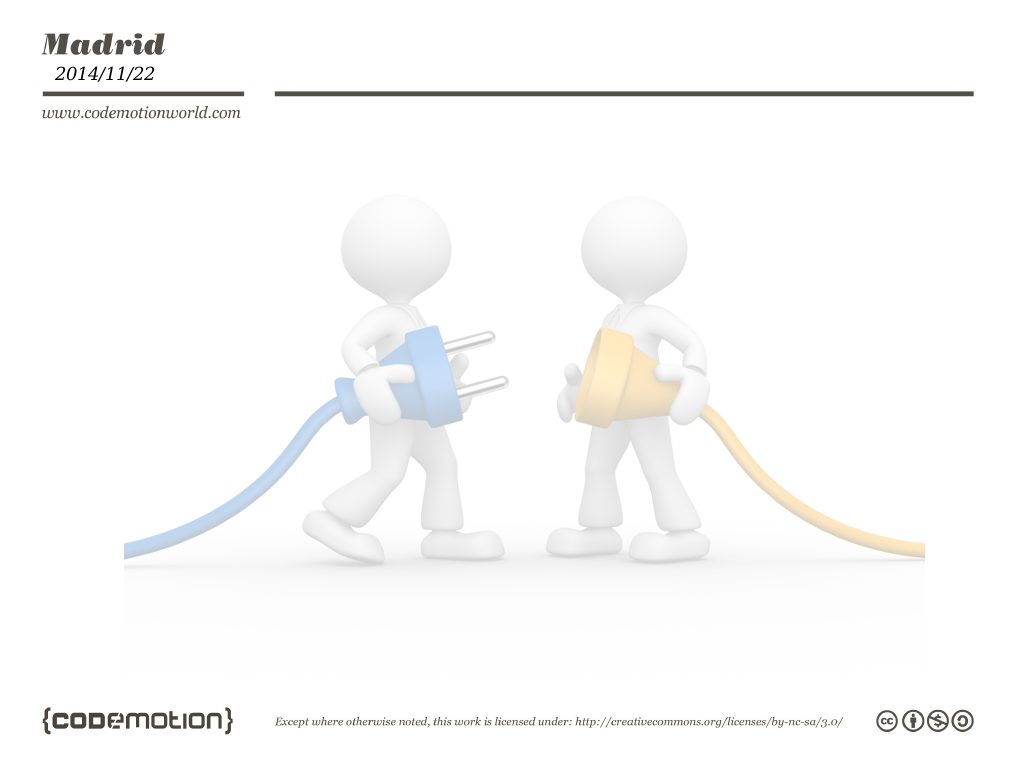
\includegraphics[width=\paperwidth]{jenkins-get-new-version-4-bg.png}
};
\node[shift={(4.5cm, -0.44cm)}, right] at (current page.north west) {Releasing the child module};
\end{tikzpicture}

\begin{block}{Finally}

\begin{itemize}
\item The trigger module, using \textbf{maven-versions-plugin} again, updates its own pom to point to the newly released parent pom.
\item Accordingly, uses \textbf{maven-release-plugin} to build all required artifacts and tag the new version: $V$.
\item For each commit, (at least) two artifacts are generated: parent-pom-$V$ and module-$V$.
\end{itemize}
\end{block}
\end{frame}
} % background


{
\setbeamertemplate{navigation symbols}{}
\begin{frame}[label=sec-6-8]{}
\begin{tikzpicture}[remember picture,overlay]
\node[at=(current page.center)] {

\includegraphics[width=\paperwidth]{jenkins-get-new-version-4b-bg.png}
};
\node[shift={(4.5cm, -0.44cm)}, right] at (current page.north west) {};
\end{tikzpicture}

\end{frame}
} % background

{
\setbeamertemplate{navigation symbols}{}
\begin{frame}[label=sec-6-9]{}
\begin{tikzpicture}[remember picture,overlay]
\node[at=(current page.center)] {
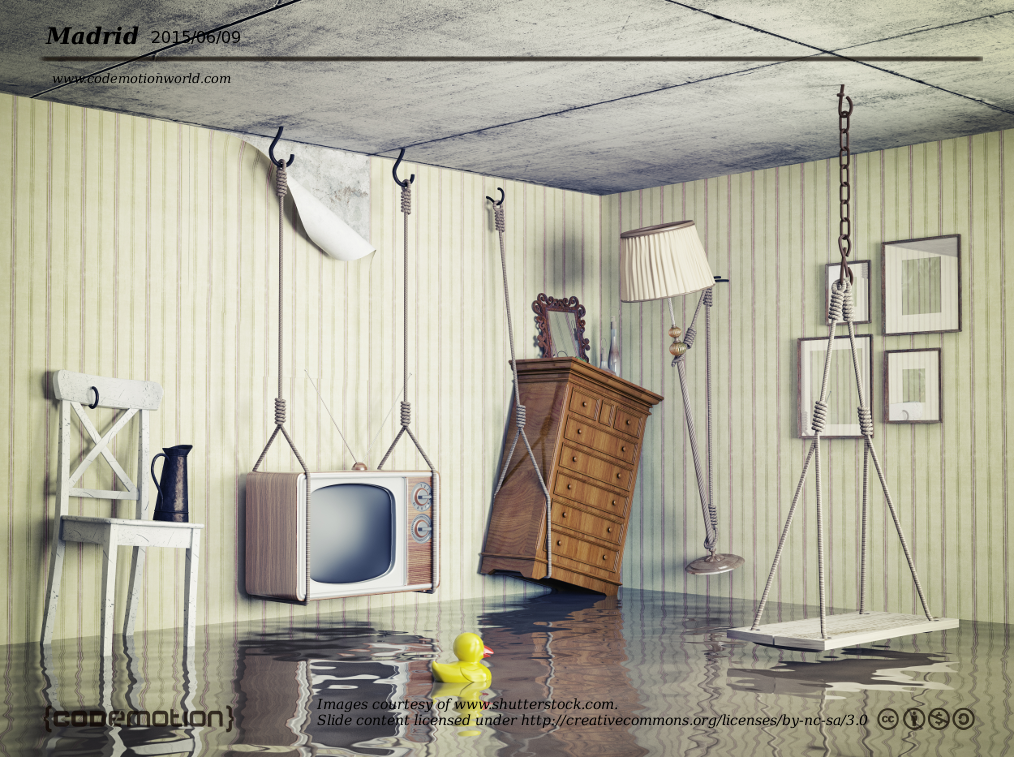
\includegraphics[width=\paperwidth]{jenkins-get-new-version-4c-bg.png}
};
\node[shift={(4.5cm, -0.44cm)}, right] at (current page.north west) {};
\end{tikzpicture}

\begin{columns}
\begin{column}{0.6\textwidth}
\begin{quotation} %% 

\end{quotation}
\end{column}
\end{columns}
\end{frame}
} % background



{
\setbeamertemplate{navigation symbols}{}
\begin{frame}[label=sec-6-10]{\textit{get-new-version} job fix}
\begin{tikzpicture}[remember picture,overlay]
\node[at=(current page.center)] {
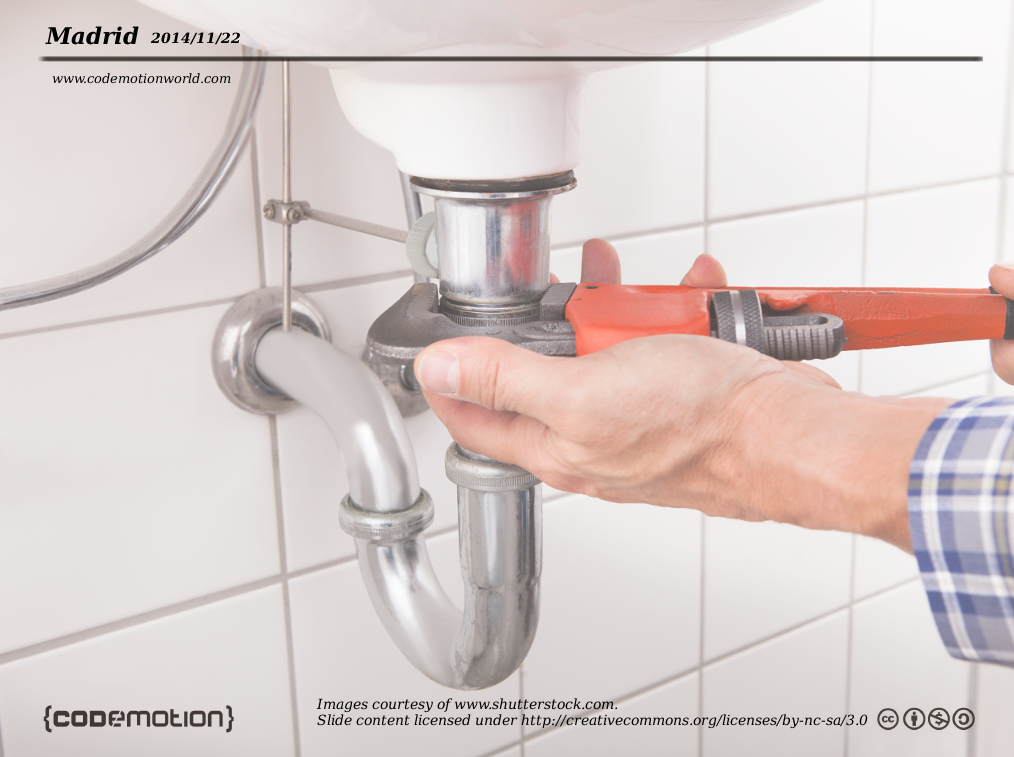
\includegraphics[width=\paperwidth]{jenkins-get-new-version-5-bg.png}
};
\node[shift={(4.5cm, -0.44cm)}, right] at (current page.north west) {\textit{get-new-version} job fix};
\end{tikzpicture}

\begin{block}{Maven Embedded is too embedded}

\begin{itemize}
\item Maven jobs in Jenkins run Maven Embedded engine.
\item Maven annotates parent jobs as dependencies in the dependency graph.
\item For \textit{get-new-version} to work, it cannot be a Maven job: It has to call Maven from the command line.
\item Otherwise, it triggers an infinite loop of downstream jobs.
\end{itemize}
\end{block}
\end{frame}
} % background


\section{Docker}
\label{sec-7}

{
\setbeamertemplate{navigation symbols}{}
\begin{frame}[label=sec-7-1]{}
\begin{tikzpicture}[remember picture,overlay]
\node[at=(current page.center)] {
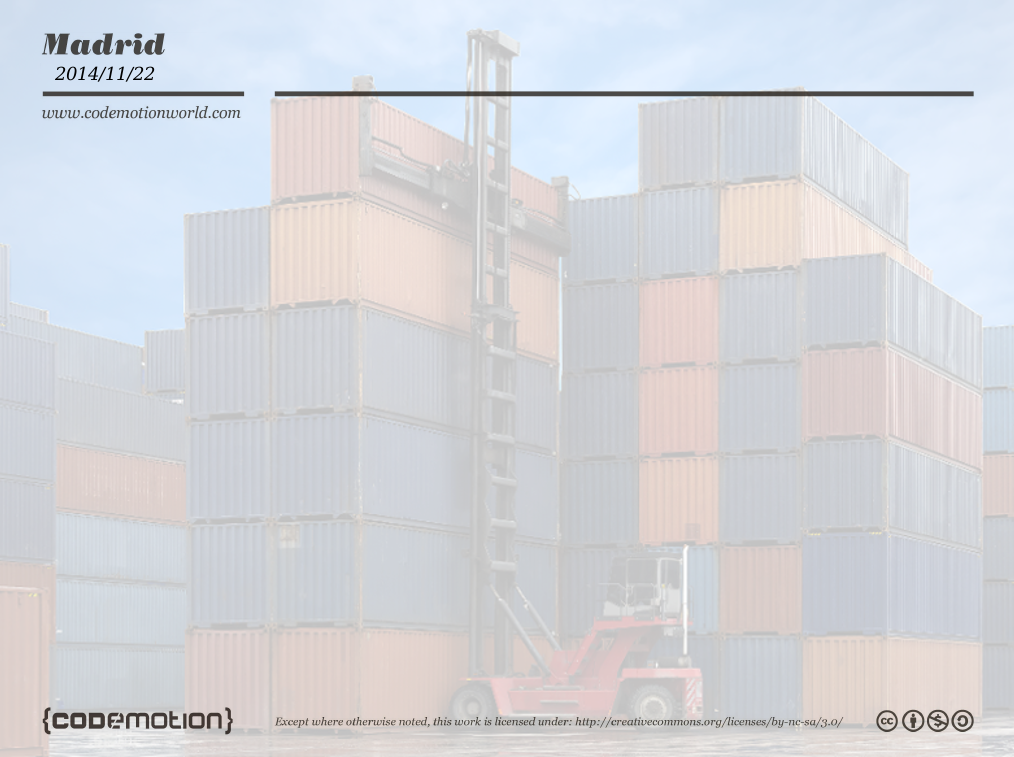
\includegraphics[width=\paperwidth]{docker-definition-bg.png}
};
\node[shift={(4.5cm, -0.44cm)}, right] at (current page.north west) {};
\end{tikzpicture}

\begin{columns}
\begin{column}{0.5\textwidth}

\textit{``An open platform for distributed applications for developers and sysadmins.''}
\end{column}

\begin{column}{0.5\textwidth}

\includegraphics[width=100]{docker-whale-home-logo.png}

\url{http://www.docker.com}
\end{column}
\end{columns}
\end{frame}
} % background

{
\setbeamertemplate{navigation symbols}{}
\begin{frame}[label=sec-7-2]{Docker}
\begin{tikzpicture}[remember picture,overlay]
\node[at=(current page.center)] {
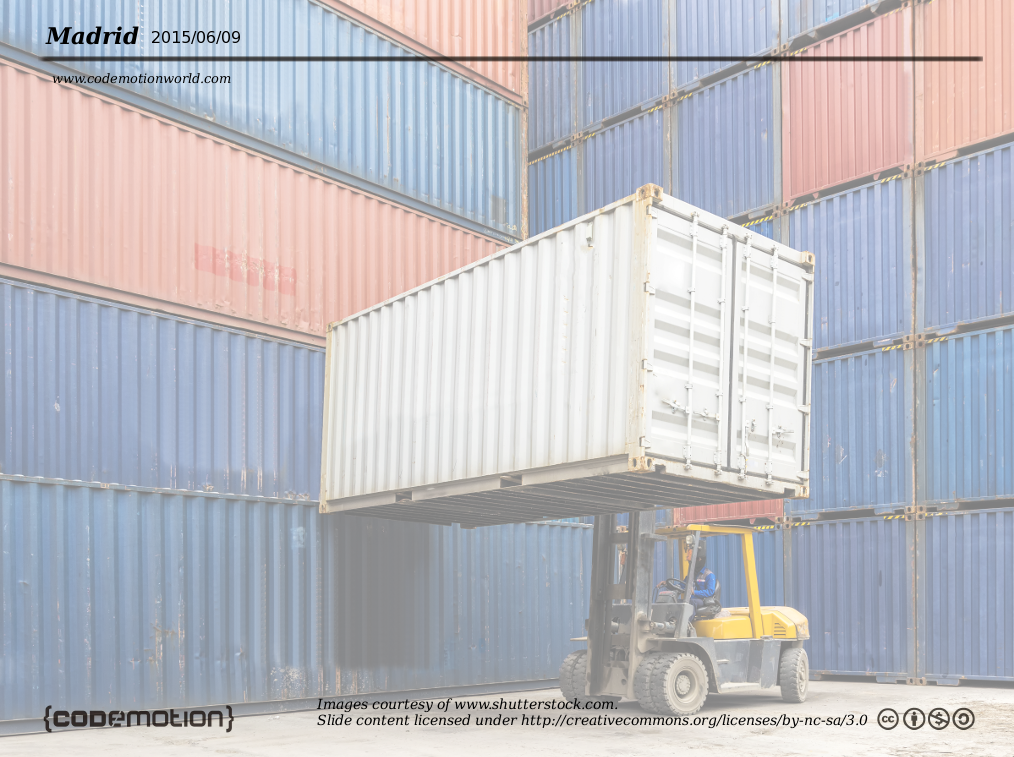
\includegraphics[width=\paperwidth]{docker-definition-2-bg.png}
};
\node[shift={(4.5cm, -0.44cm)}, right] at (current page.north west) {Docker};
\end{tikzpicture}

\begin{block}{Docker}

``The Docker Engine container comprises just the application and its dependencies. It runs as an isolated process in userspace on the host operating system, sharing the kernel with other containers. Thus, it enjoys the resource isolation and allocation benefits of VMs but is much more portable and efficient.''
\end{block}
\end{frame}
} % background

{
\setbeamertemplate{navigation symbols}{}
\begin{frame}[label=sec-7-3]{Docker Concepts (1)}
\begin{tikzpicture}[remember picture,overlay]
\node[at=(current page.center)] {
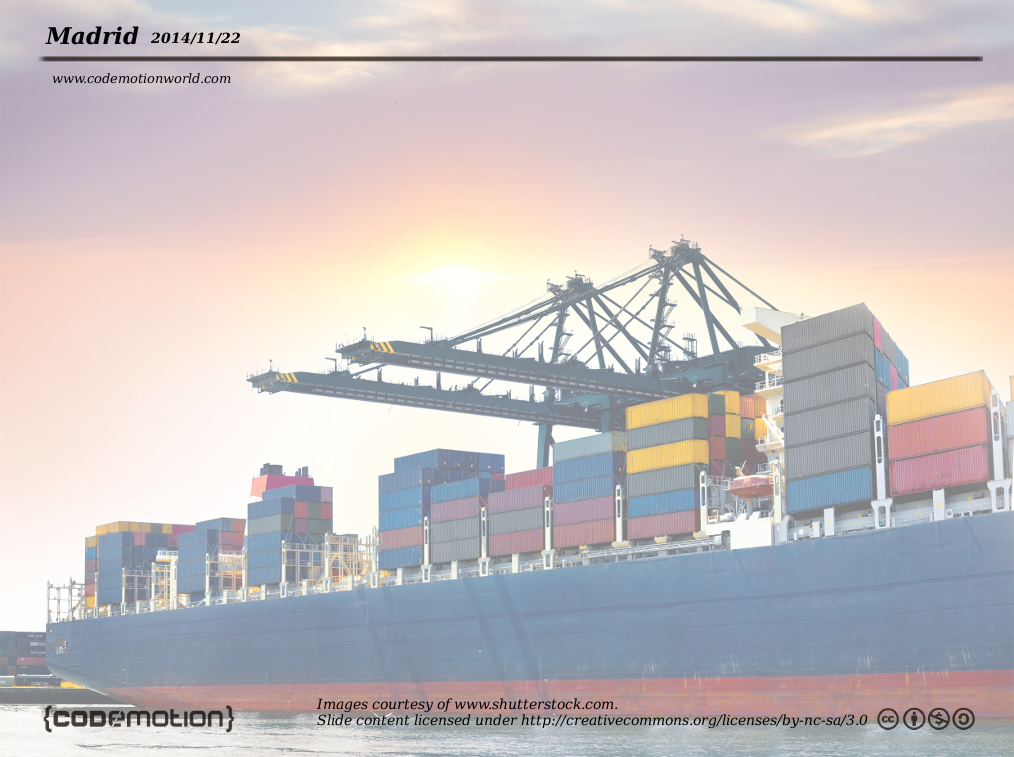
\includegraphics[width=\paperwidth]{docker-concepts-1-bg.png}
};
\node[shift={(4.5cm, -0.44cm)}, right] at (current page.north west) {Docker Concepts (1)};
\end{tikzpicture}

\begin{block}{Packaging applications}

\begin{itemize}
\item \textbf{Image}: Packaged application and dependencies. Ready to launch.
\item \textbf{Container}: An isolated (process, memory, network, etc.) environment, running an \textit{image}.
\item \textbf{Volume}: A folder within a container, accessible from the host. Can be directly mapped to a folder in the host.
\end{itemize}
\end{block}
\end{frame}
} % background

{
\setbeamertemplate{navigation symbols}{}
\begin{frame}[label=sec-7-4]{Docker Concepts (2)}
\begin{tikzpicture}[remember picture,overlay]
\node[at=(current page.center)] {
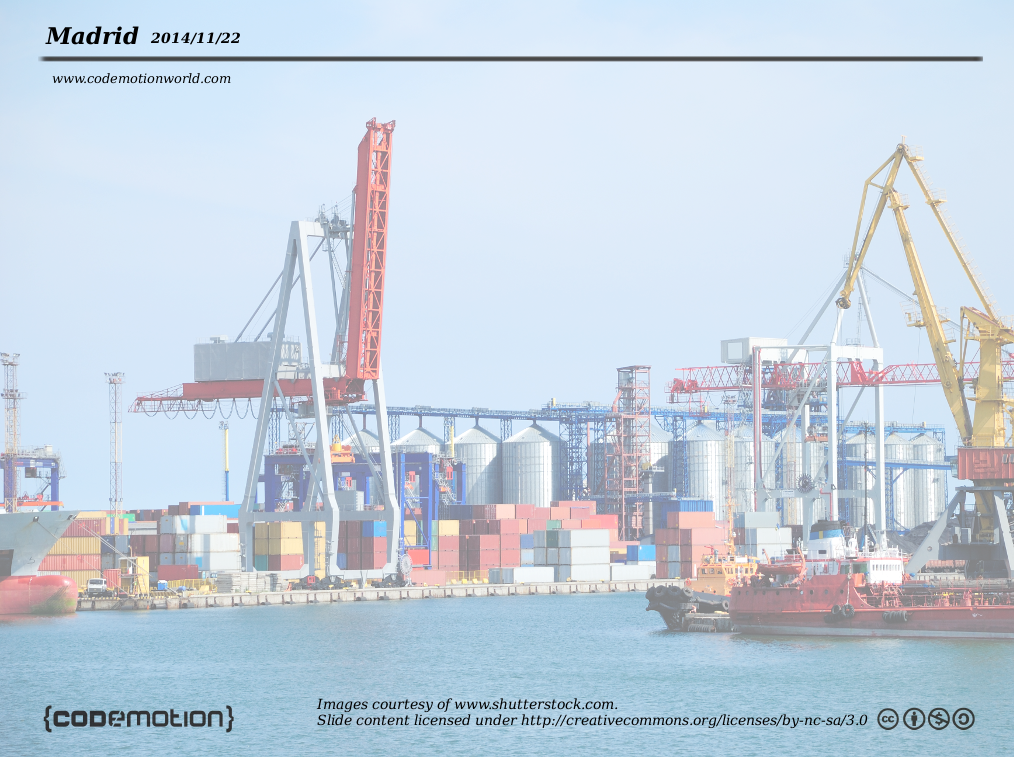
\includegraphics[width=\paperwidth]{docker-concepts-2-bg.png}
};
\node[shift={(4.5cm, -0.44cm)}, right] at (current page.north west) {Docker Concepts (2)};
\end{tikzpicture}

\begin{block}{Running applications}

\begin{itemize}
\item \textbf{Link}: Docker mechanism to help containers communicate with each other. It's defined as \texttt{--link container:alias}:
\begin{itemize}
\item \textit{container}: the name of the external, already running container,
\item \textit{alias}: the name used locally in the new container, pointing to the external container. Docker adds it to /etc/hosts, and defines some environment properties.
\end{itemize}
\item \textbf{Exposed port}: Docker service can map host ports to internal ports, when the container starts.
\end{itemize}
\end{block}
\end{frame}
} % background

{
\setbeamertemplate{navigation symbols}{}
\begin{frame}[label=sec-7-5]{phusion-baseimage}
\begin{tikzpicture}[remember picture,overlay]
\node[at=(current page.center)] {
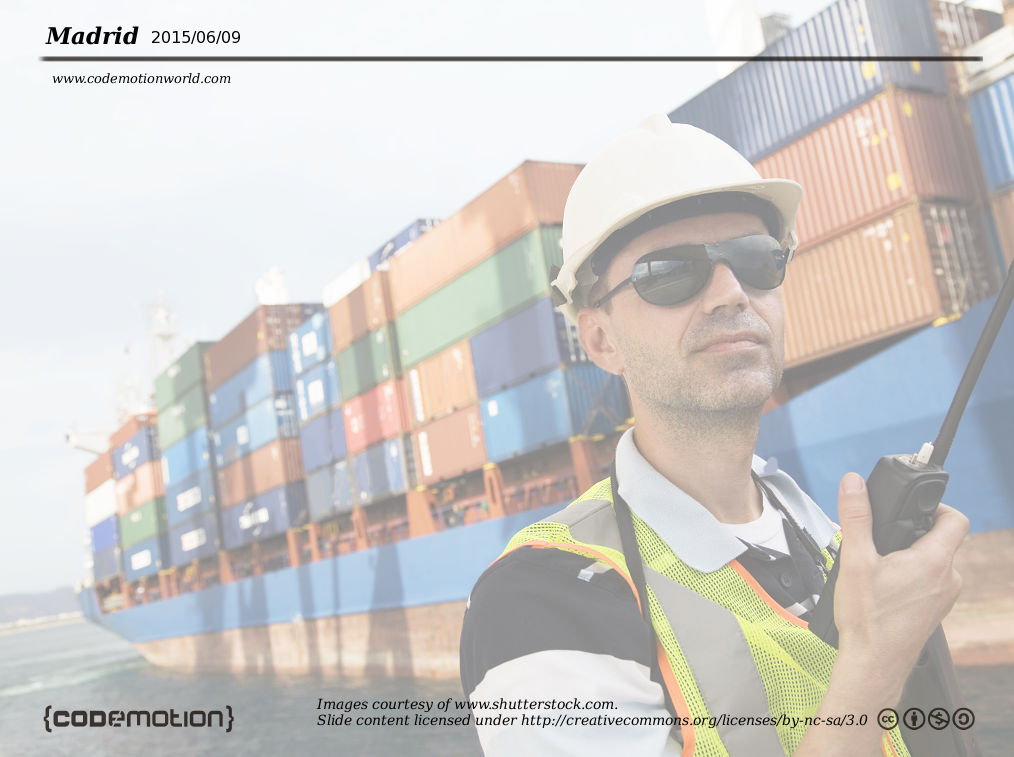
\includegraphics[width=\paperwidth]{docker-phusion-baseimage-bg.png}
};
\node[shift={(4.5cm, -0.44cm)}, right] at (current page.north west) {phusion-baseimage};
\end{tikzpicture}

\begin{block}{Cleaning things up}

\begin{itemize}
\item A minimal Ubuntu base image modified for Docker-friendliness.
\item Takes care of the problem of:
\begin{itemize}
\item Zombie processes,
\item Logger daemon,
\item Cron jobs.
\end{itemize}
\item Motivation explained in their website: ``Your Docker image might be broken without you knowing it''
\end{itemize}
\url{https://phusion.github.io/baseimage-docker/}
\end{block}
\end{frame}
} % background

{
\setbeamertemplate{navigation symbols}{}
\begin{frame}[label=sec-7-6]{Dockerfile templates}
\begin{tikzpicture}[remember picture,overlay]
\node[at=(current page.center)] {

\includegraphics[width=\paperwidth]{docker-dockerfile-templates-bg.png}
};
\node[shift={(4.5cm, -0.44cm)}, right] at (current page.north west) {Dockerfile templates};
\end{tikzpicture}

\begin{block}{Variables in Dockerfiles}

\begin{itemize}
\item Based on wking's approach and code for Gentoo-based images:
\url{https://github.com/wking/dockerfile}
\item Modified for phusion-baseimage.
\item Enhanced with in-house bash scripting framework: dry-wit.
\item Allows placeholders in Dockerfiles.
\end{itemize}
\end{block}
\end{frame}
} % background

\section{Shipyard}
\label{sec-8}

{
\setbeamertemplate{navigation symbols}{}
\begin{frame}[label=sec-8-1]{Shipyard}
\begin{tikzpicture}[remember picture,overlay]
\node[at=(current page.center)] {
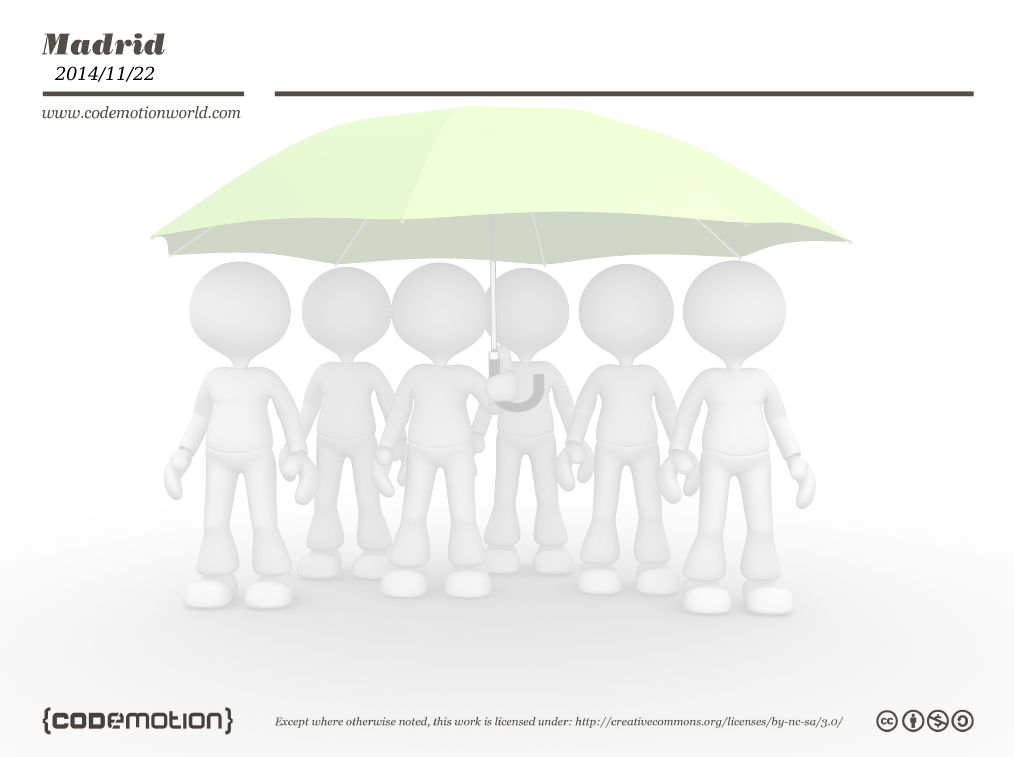
\includegraphics[width=\paperwidth]{shipyard-definition-bg.png}
};
\node[shift={(4.5cm, -0.44cm)}, right] at (current page.north west) {Shipyard};
\end{tikzpicture}

\begin{columns}
\begin{column}{0.6\textwidth}

\textit{``Built on the Docker cluster management toolkit Citadel, Shipyard gives you the ability to manage Docker resources including containers, hosts and more.}

\textit{Shipyard differs from other management applications in that it promotes composability. At the core, Shipyard only manages Docker (containers, etc). However, using "Extension Images" you can add functionality such as application routing and load balancing, centralized logging, deployment and more.''}
\end{column}

\begin{column}{0.4\textwidth}

\includegraphics[width=100]{shipyard-logo.png}

\small{http://shipyard-project.com}
\end{column}
\end{columns}
\end{frame}
} % background

{
\setbeamertemplate{navigation symbols}{}
\begin{frame}[label=sec-8-2]{}
\begin{tikzpicture}[remember picture,overlay]
\node[at=(current page.center)] {
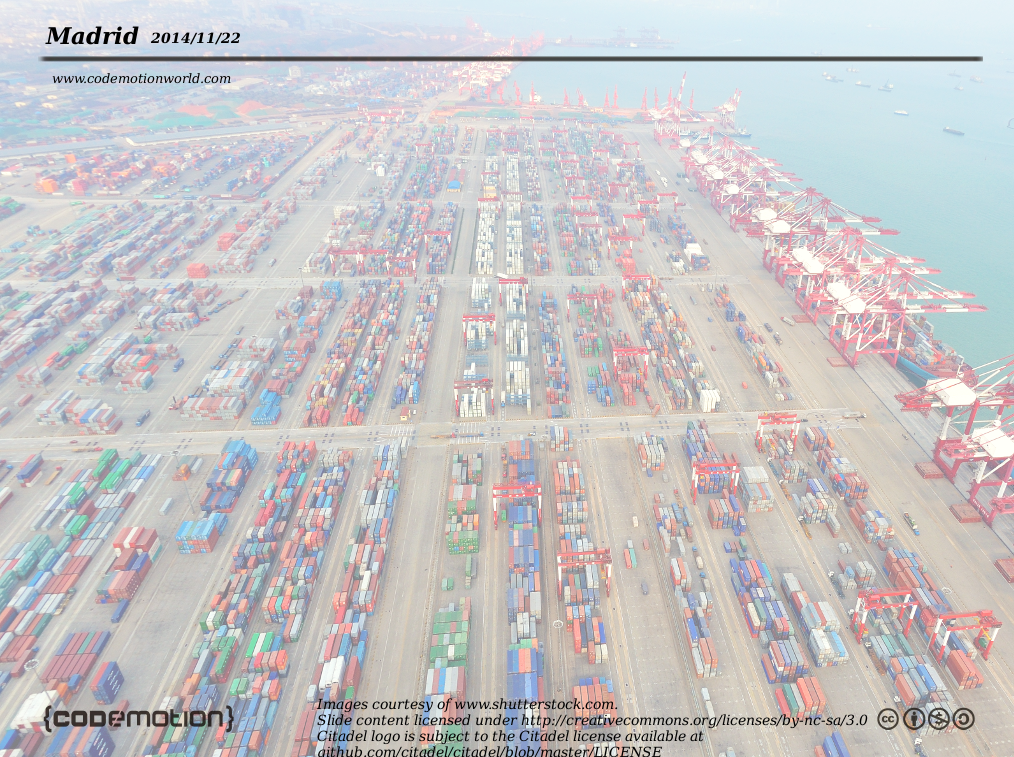
\includegraphics[width=\paperwidth]{shipyard-citadel-bg.png}
};
\node[shift={(4.5cm, -0.44cm)}, right] at (current page.north west) {};
\end{tikzpicture}

\begin{columns}
\begin{column}{0.6\textwidth}

\textit{``Citadel is a toolkit for scheduling containers on a Docker cluster.''}
\end{column}

\begin{column}{0.4\textwidth}

\includegraphics[width=100]{citadel-logo.png}

\small{http://citadeltoolkit.org}
\end{column}
\end{columns}
\end{frame}
} % background

\section{Puppet}
\label{sec-9}

{
\setbeamertemplate{navigation symbols}{}
\begin{frame}[label=sec-9-1]{Puppet}
\begin{tikzpicture}[remember picture,overlay]
\node[at=(current page.center)] {
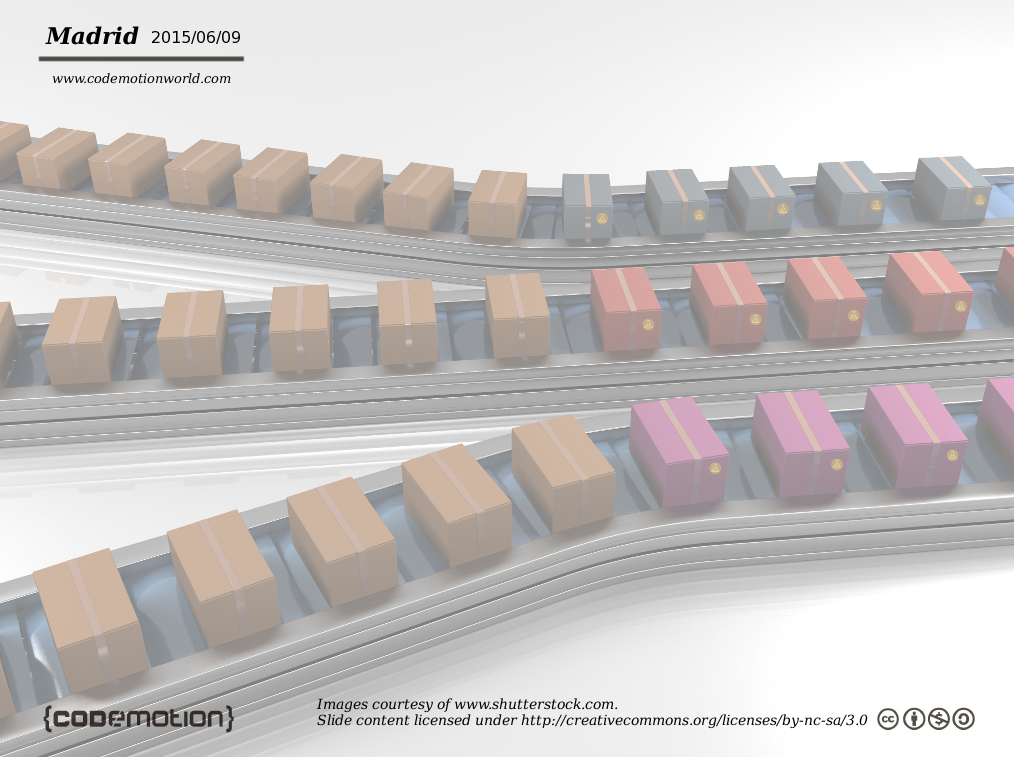
\includegraphics[width=\paperwidth]{puppet-definition-bg.png}
};
\node[shift={(4.5cm, -0.44cm)}, right] at (current page.north west) {Puppet};
\end{tikzpicture}

\begin{columns}
\begin{column}{0.6\textwidth}

\textit{``Puppet manages your servers: you describe machine configurations in an easy-to-read declarative language, and Puppet will bring your systems into the desired state and keep them there.''}
\end{column}

\begin{column}{0.4\textwidth}

\includegraphics[width=100]{puppet-logo.png}

\small{http://www.puppetlabs.com}
\end{column}
\end{columns}
\end{frame}
} % background

{
\setbeamertemplate{navigation symbols}{}
\begin{frame}[label=sec-9-2]{Puppet}
\begin{tikzpicture}[remember picture,overlay]
\node[at=(current page.center)] {
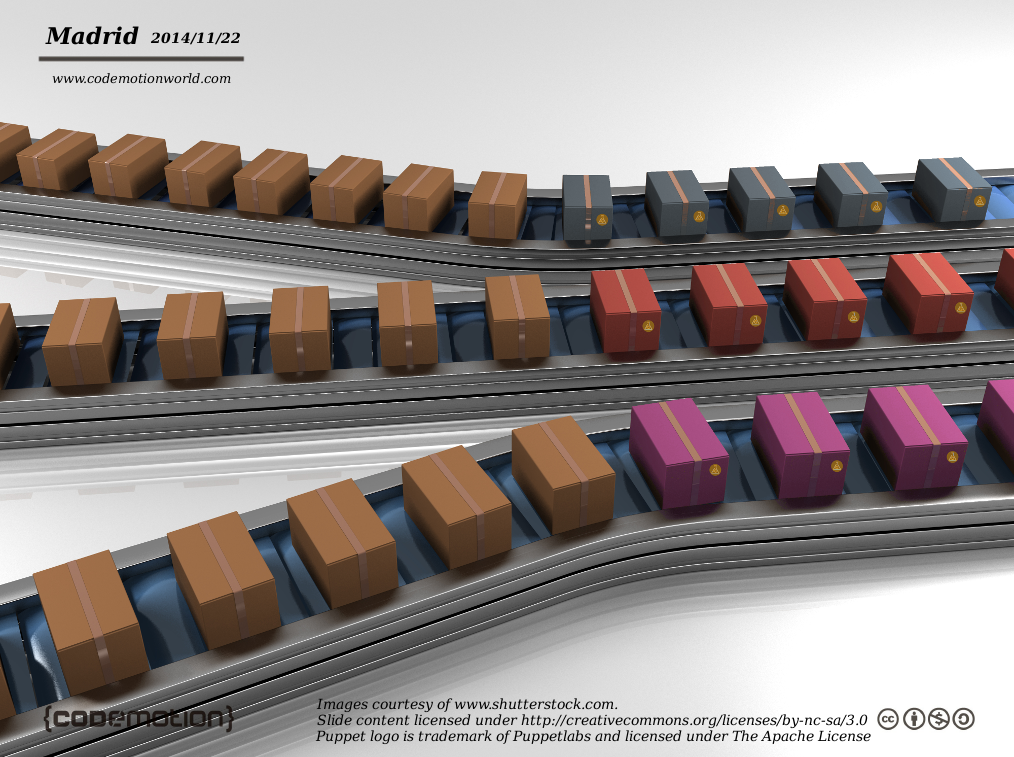
\includegraphics[width=\paperwidth]{puppet-definition-1-bg.png}
};
\node[shift={(4.5cm, -0.44cm)}, right] at (current page.north west) {Puppet};
\end{tikzpicture}

\end{frame}
} % background

{
\setbeamertemplate{navigation symbols}{}
\begin{frame}[label=sec-9-3]{Puppet on guests}
\begin{tikzpicture}[remember picture,overlay]
\node[at=(current page.center)] {
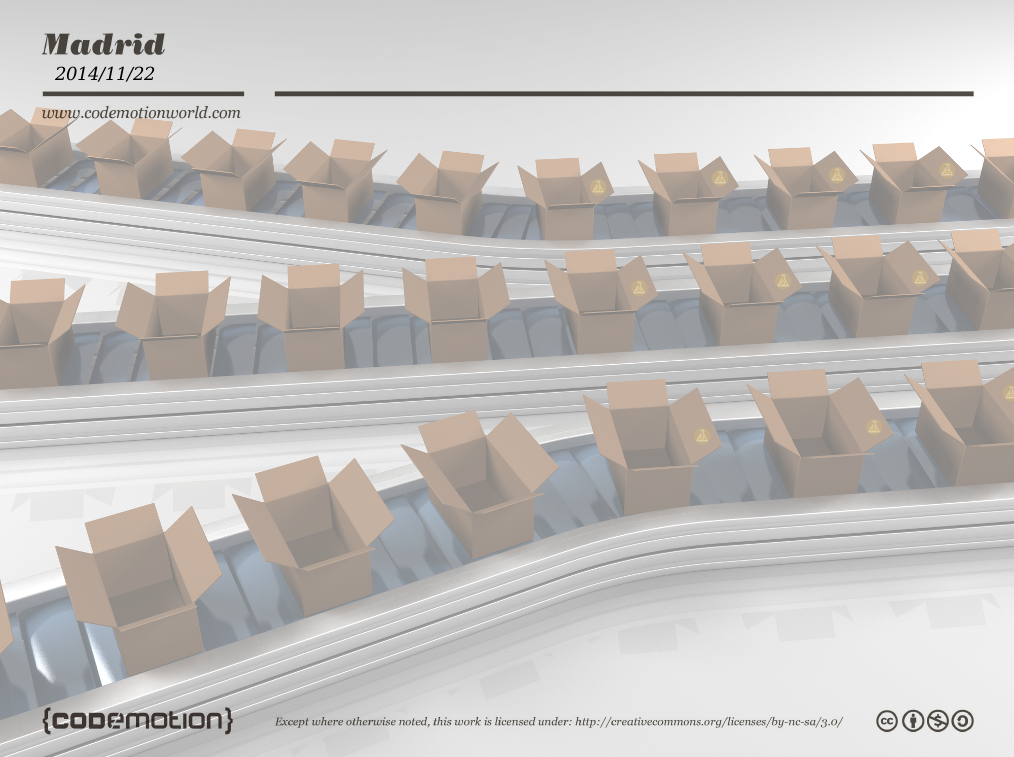
\includegraphics[width=\paperwidth]{puppet-on-guests-bg.png}
};
\node[shift={(4.5cm, -0.44cm)}, right] at (current page.north west) {Puppet on guests};
\end{tikzpicture}


\begin{columns}
\begin{column}{0.5\textwidth}
\begin{block}{Pros}

\begin{itemize}
\item Images can be deployed anywhere.
\item It doesn't require a convention to map host volumes or data containers.
\item Containers can respond to changes propagated via Puppet.
\end{itemize}
\end{block}
\end{column}

\begin{column}{0.5\textwidth}
\begin{block}{Cons}

\begin{itemize}
\item Containers take much longer to start.
\item Automatic generation, auto-sign, and auto-accept SSL certificates.
\item Puppet infrastructure required in production.
\end{itemize}
\end{block}
\end{column}
\end{columns}
\end{frame}
} % background

{
\setbeamertemplate{navigation symbols}{}
\begin{frame}[label=sec-9-4]{Puppet on hosts}
\begin{tikzpicture}[remember picture,overlay]
\node[at=(current page.center)] {
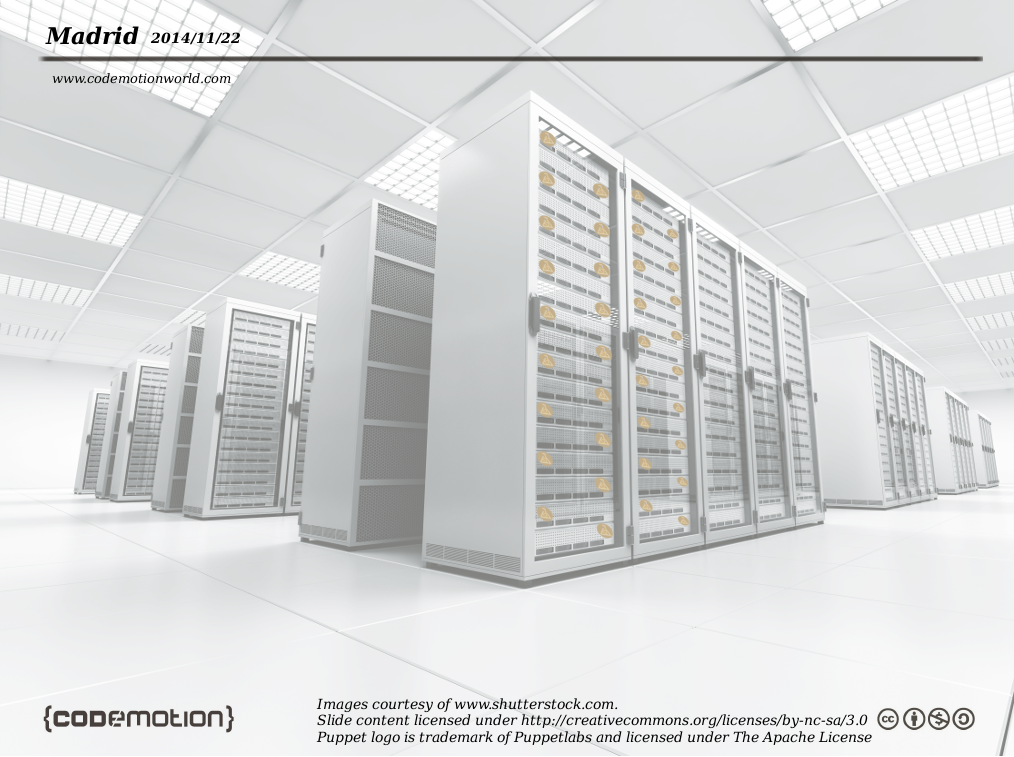
\includegraphics[width=\paperwidth]{puppet-on-hosts-bg.png}
};
\node[shift={(4.5cm, -0.44cm)}, right] at (current page.north west) {Puppet on hosts};
\end{tikzpicture}

\begin{columns}
\begin{column}{0.5\textwidth}
\begin{block}{Pros}

\begin{itemize}
\item Containers are staless.
\item Containers launch fast.
\end{itemize}
\end{block}
\end{column}

\begin{column}{0.5\textwidth}
\begin{block}{Cons}

\begin{itemize}
\item Containers need to be prepared to read their configuration from plain files.
\item The command for launching containers depends on Puppet configuration for that host.
\item Puppet infrastructure required in production.
\end{itemize}
\end{block}
\end{column}
\end{columns}
\end{frame}
} % background

{
\setbeamertemplate{navigation symbols}{}
\begin{frame}[label=sec-9-5]{Puppet to build data-container images}
\begin{tikzpicture}[remember picture,overlay]
\node[at=(current page.center)] {
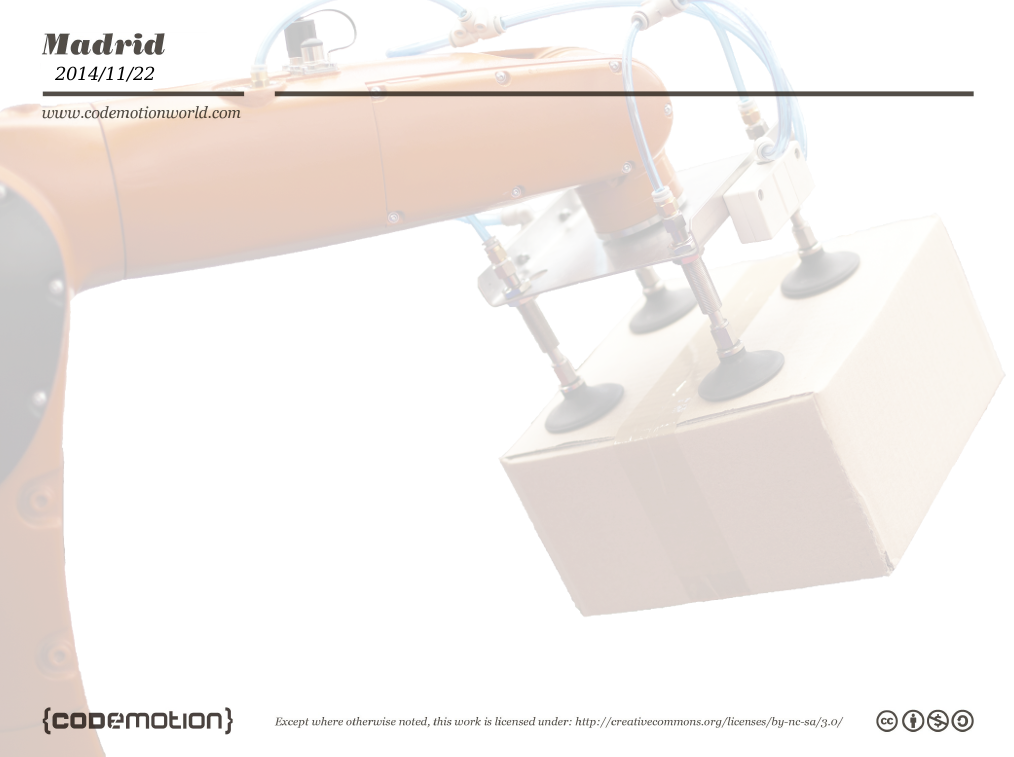
\includegraphics[width=\paperwidth]{puppet-to-build-data-container-images-bg.png}
};
\node[shift={(4.5cm, -0.44cm)}, right] at (current page.north west) {Puppet to build data-container images};
\end{tikzpicture}

\begin{columns}
\begin{column}{0.5\textwidth}
\begin{block}{Pros}

\begin{itemize}
\item Puppet sets up the configuration for environment-aware images.
\item No Puppet needed in production: just links to data containers.
\item Launching containers do not depend on the host.
\end{itemize}
\end{block}
\end{column}

\begin{column}{0.5\textwidth}
\begin{block}{Cons}

\begin{itemize}
\item SSL certificate magic takes place on intermediate Docker images.
\item A change in Puppet requires rebuilding the images, replacing the data-containers, and probably the application containers as well.
\end{itemize}
\end{block}
\end{column}
\end{columns}
\end{frame}
} % background

{
\setbeamertemplate{navigation symbols}{}
\begin{frame}[label=sec-9-6]{Puppet to manage data-container images}
\begin{tikzpicture}[remember picture,overlay]
\node[at=(current page.center)] {
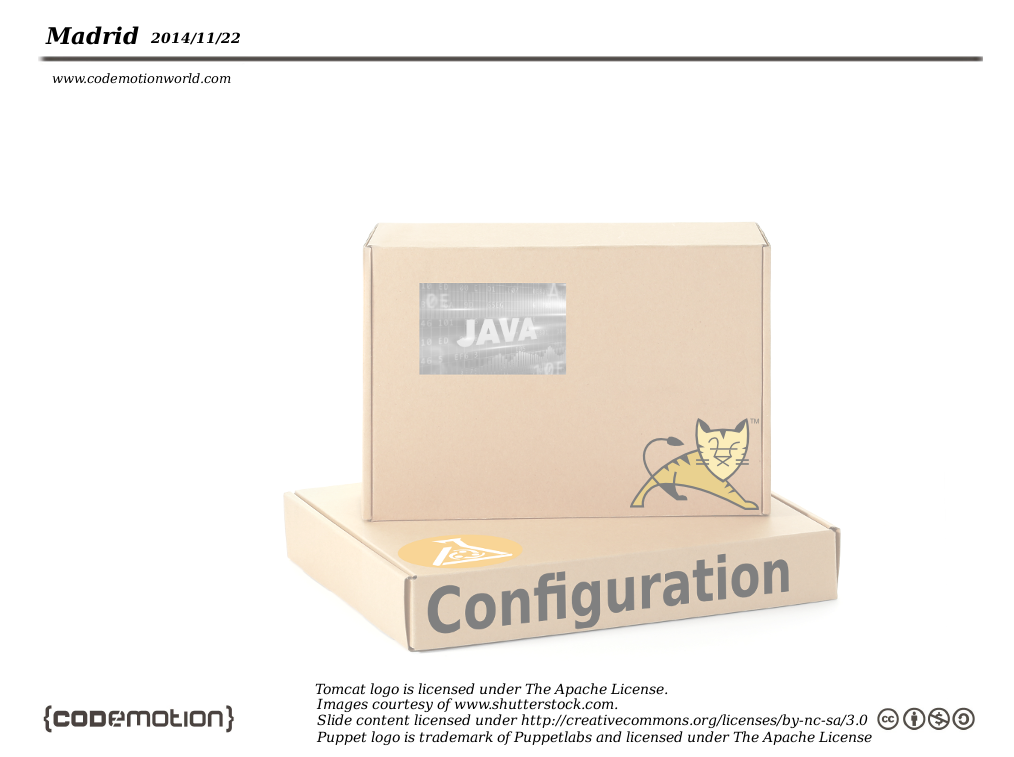
\includegraphics[width=\paperwidth]{puppet-to-manage-data-container-images-1-bg.png}
};
\node[shift={(4.5cm, -0.44cm)}, right] at (current page.north west) {Puppet to manage data-container images};
\end{tikzpicture}

\end{frame}
} % background

{
\setbeamertemplate{navigation symbols}{}
\begin{frame}[label=sec-9-7]{Environment isolated in data containers}
\begin{tikzpicture}[remember picture,overlay]
\node[at=(current page.center)] {
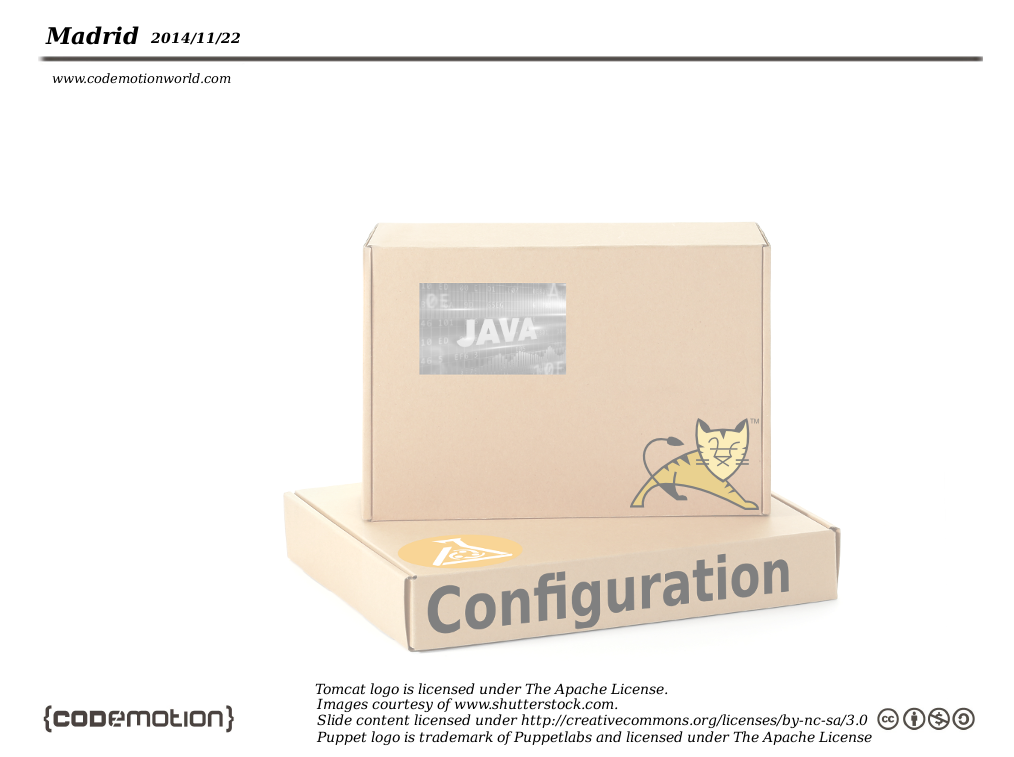
\includegraphics[width=\paperwidth]{puppet-to-manage-data-container-images-1-bg.png}
};
\node[shift={(4.5cm, -0.44cm)}, right] at (current page.north west) {Environment isolated in data containers};
\end{tikzpicture}

\begin{columns}
\begin{column}{0.5\textwidth}
\begin{block}{Pros}

\begin{itemize}
\item Data containers launch the Puppet agent: their configuration can evolve over time.
\item Puppet sets up the configuration depending on the environment.
\item Launching containers do not depend on the host.
\end{itemize}
\end{block}
\end{column}

\begin{column}{0.5\textwidth}
\begin{block}{Cons}

\begin{itemize}
\item Puppet infrastructure needed in production.
\item SSL certificate magic takes place on data containers.
\end{itemize}
\end{block}
\end{column}
\end{columns}
\end{frame}
} % background

\section{MCollective}
\label{sec-10}

{
\setbeamertemplate{navigation symbols}{}
\begin{frame}[label=sec-10-1]{MCollective}
\begin{tikzpicture}[remember picture,overlay]
\node[at=(current page.center)] {

\includegraphics[width=\paperwidth]{mcollective-definition-bg.png}
};
\node[shift={(4.5cm, -0.44cm)}, right] at (current page.north west) {MCollective};
\end{tikzpicture}

\begin{columns}
\begin{column}{0.6\textwidth}

\textit{``MCollective is a powerful orchestration framework.}

\textit{Run actions on thousands of servers simultaneously, using existing plugins or writing your own.''}
\end{column}

\begin{column}{0.4\textwidth}


\includegraphics[width=100]{mcollective-logo.png}

\small{http://www.puppetlabs.com}
\end{column}
\end{columns}
\end{frame}
} % background


{
\setbeamertemplate{navigation symbols}{}
\begin{frame}[label=sec-10-2]{ssh in a loop (1)}
\begin{tikzpicture}[remember picture,overlay]
\node[at=(current page.center)] {
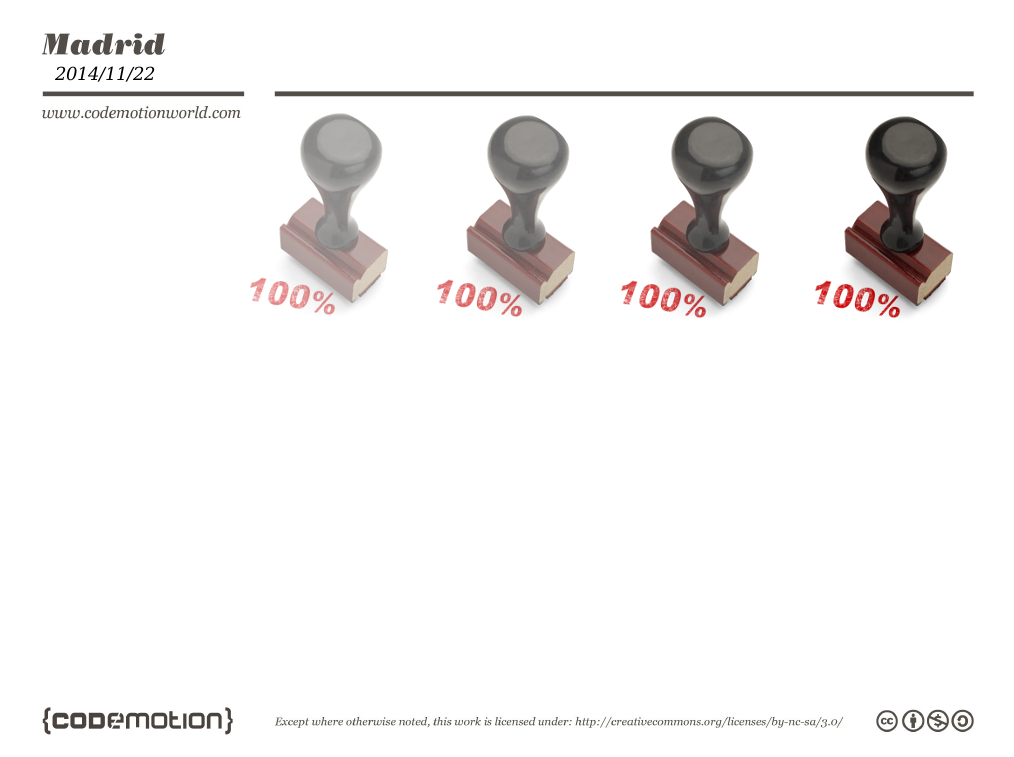
\includegraphics[width=\paperwidth]{mcollective-ssh-in-a-loop-1-bg.png}
};
\node[shift={(4.5cm, -0.44cm)}, right] at (current page.north west) {ssh in a loop (1)};
\end{tikzpicture}

\begin{block}{Pros}

\begin{itemize}
\item Simple and straightforward.
\item Fast enough up to a certain number of hosts.
\item Easy and cheap to adapt to perform different tasks.
\item Scriptable.
\end{itemize}
\end{block}
\end{frame}
} % background

{
\setbeamertemplate{navigation symbols}{}
\begin{frame}[label=sec-10-3]{ssh in a loop (2)}
\begin{tikzpicture}[remember picture,overlay]
\node[at=(current page.center)] {
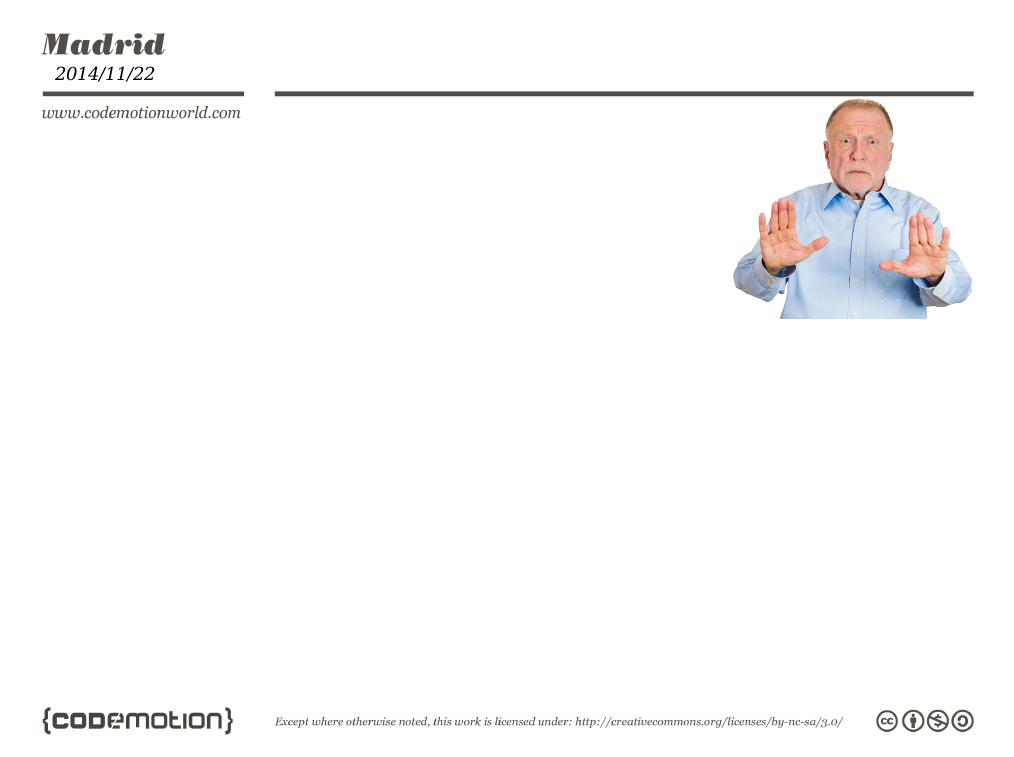
\includegraphics[width=\paperwidth]{mcollective-ssh-in-a-loop-2-bg.png}
};
\node[shift={(4.5cm, -0.44cm)}, right] at (current page.north west) {ssh in a loop (2)};
\end{tikzpicture}

\begin{block}{Cons}

\begin{itemize}
\item Scripts with hard-coded host names or IPs.
\item Requires way too much information about the production environment.
\item Cannot easily run remote commands which expect some kind of interaction.
\item When the number of host grows, the risk of overlook reported problems increases.
\item Requires dealing with account permissions, SSO, etc.
\end{itemize}
\end{block}
\end{frame}
} % background

{
\setbeamertemplate{navigation symbols}{}
\begin{frame}[label=sec-10-4]{MCollective}
\begin{tikzpicture}[remember picture,overlay]
\node[at=(current page.center)] {
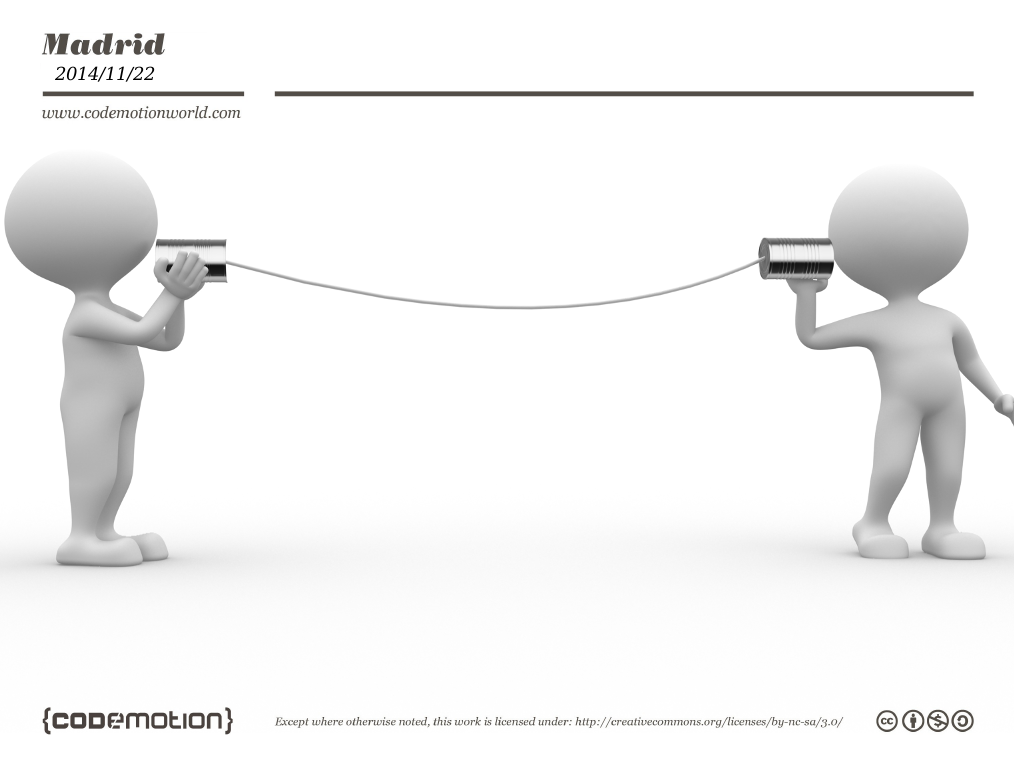
\includegraphics[width=\paperwidth]{mcollective-bg.png}
};
\node[shift={(4.5cm, -0.44cm)}, right] at (current page.north west) {MCollective};
\end{tikzpicture}

\begin{columns}
\begin{column}{0.5\textwidth}
\begin{block}{Pros}

\begin{itemize}
\item Scales with the number of hosts in production.
\item Extendable via plugins.
\item Doesn't require system accounts, SSO on production hosts.
\item Puppet module available for servers.
\end{itemize}
\end{block}
\end{column}

\begin{column}{0.5\textwidth}
\begin{block}{Cons}

\begin{itemize}
\item More complex architecture.
\item Requires middleware.
\item Scaling beyond certain size requires tuning.
\item Middleware should be fault-tolerant.
\item Misconfigured setups can generate excessive traffic.
\end{itemize}
\end{block}
\end{column}
\end{columns}
\end{frame}
} % background

{
\setbeamertemplate{navigation symbols}{}
\begin{frame}[label=sec-10-5]{Architecture}
\begin{tikzpicture}[remember picture,overlay]
\node[at=(current page.center)] {
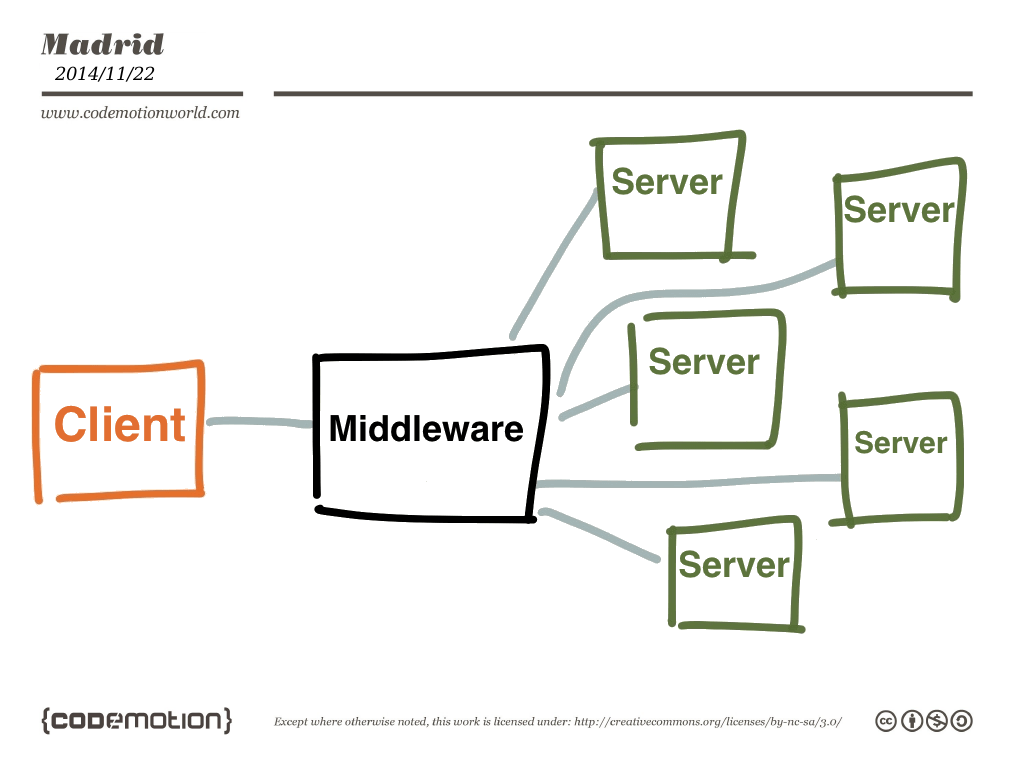
\includegraphics[width=\paperwidth]{mcollective-architecture-bg.png}
};
\node[shift={(4.5cm, -0.44cm)}, right] at (current page.north west) {Architecture};
\end{tikzpicture}

\end{frame}
} % background

{
\setbeamertemplate{navigation symbols}{}
\begin{frame}[label=sec-10-6]{Middleware}
\begin{tikzpicture}[remember picture,overlay]
\node[at=(current page.center)] {
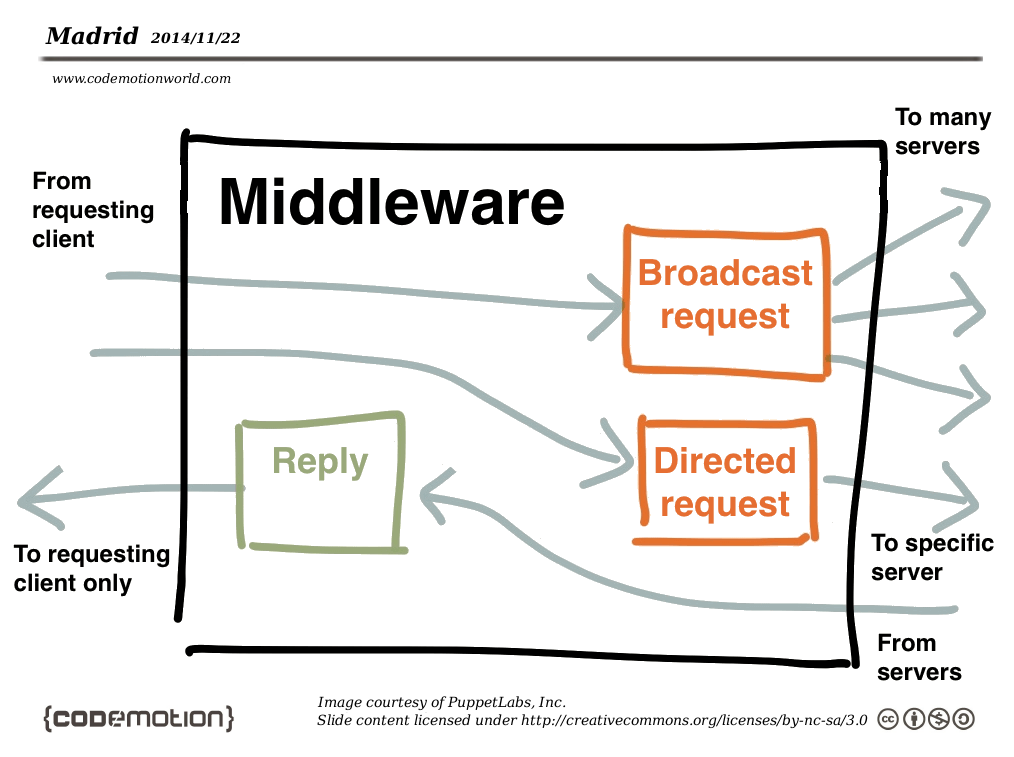
\includegraphics[width=\paperwidth]{mcollective-middleware-bg.png}
};
\node[shift={(4.5cm, -0.44cm)}, right] at (current page.north west) {Middleware};
\end{tikzpicture}

\end{frame}
} % background

\section{Next steps}
\label{sec-11}
{
\setbeamertemplate{navigation symbols}{}
\begin{frame}[label=sec-11-1]{Now what?}
\begin{tikzpicture}[remember picture,overlay]
\node[at=(current page.center)] {
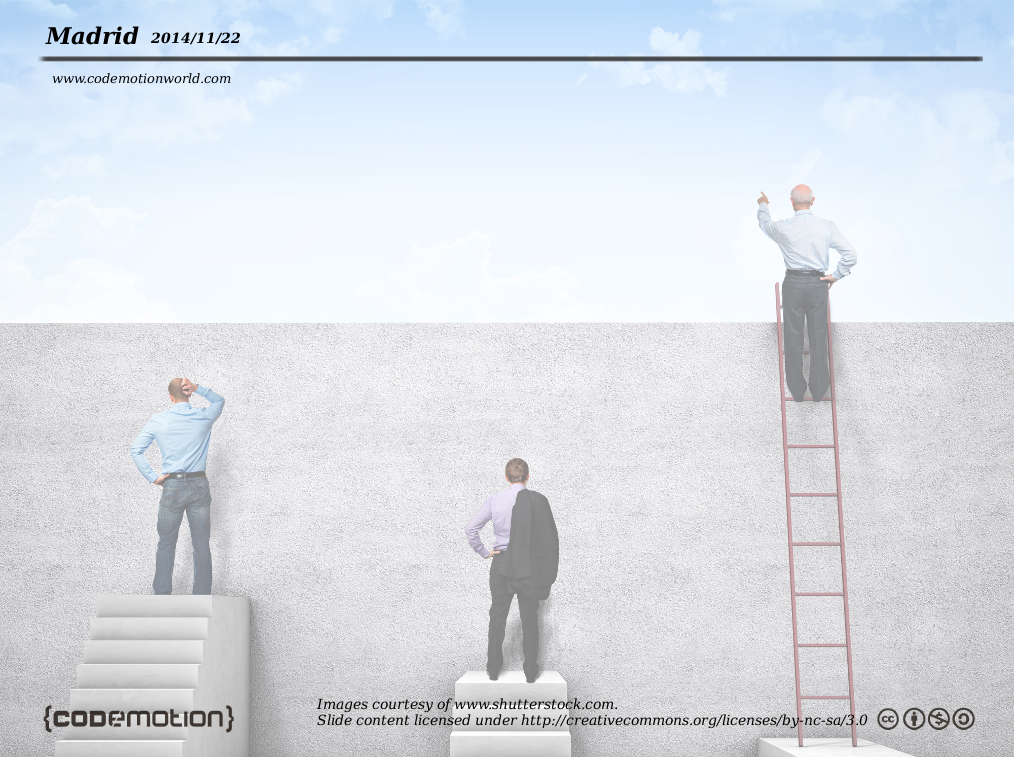
\includegraphics[width=\paperwidth]{now-what-bg.png}
};
\node[shift={(4.5cm, -0.44cm)}, right] at (current page.north west) {Now what?};
\end{tikzpicture}


\begin{block}{First things first}

\begin{itemize}
\item Clone my repos: \url{http://github.com/rydnr/dockerfile} and \url{http://github.com/rydnr/dry-wit}
\item Take \url{http://githob.com/rydnr/acmsl-jenkins-configs} as a template for \textbf{get-new-version} job.
\item Build your custom Delivery Pipeline.
\item Make Jenkins generate Docker images and push them to a private index.
\end{itemize}
\end{block}
\end{frame}
} % background

{
\setbeamertemplate{navigation symbols}{}
\begin{frame}[label=sec-11-2]{And then?}
\begin{tikzpicture}[remember picture,overlay]
\node[at=(current page.center)] {
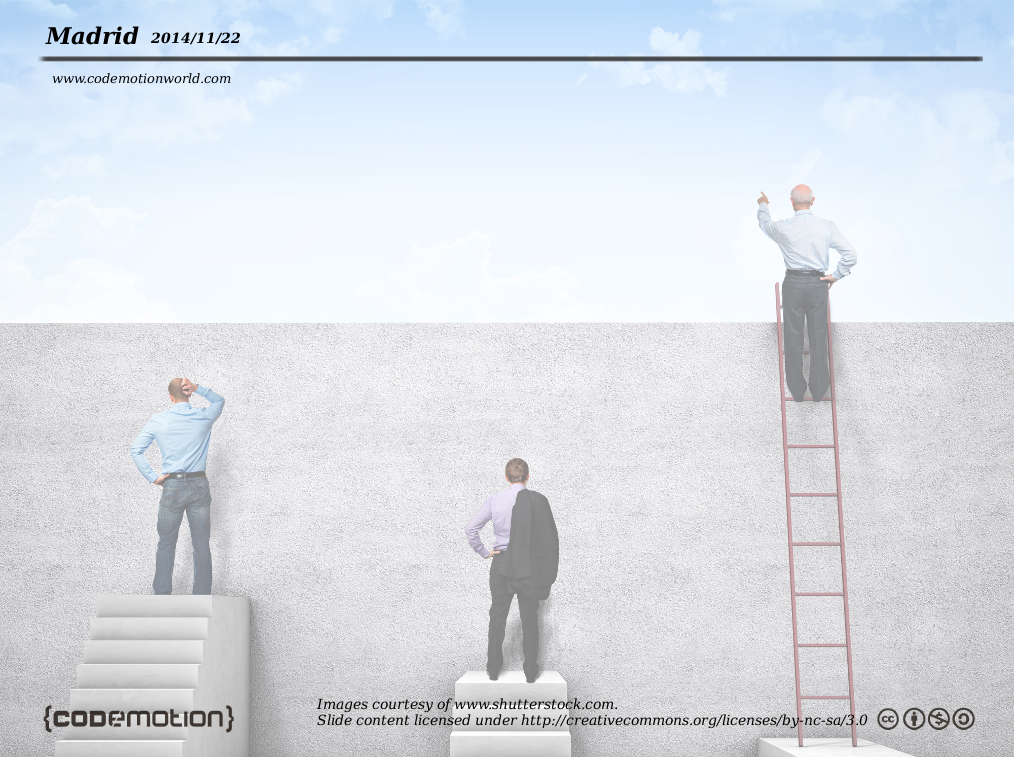
\includegraphics[width=\paperwidth]{now-what-bg.png}
};
\node[shift={(4.5cm, -0.44cm)}, right] at (current page.north west) {And then?};
\end{tikzpicture}

\begin{block}{Customize and test}

\begin{itemize}
\item Build mcollective-client and mcollective-server images.
\item Install shipyard and mcollective server agent in a test environment.
\item Launch docker containers from the mcollective client, via mcollective shell agent.
\item Try Interlock in the path to Continuous Deployment!
\end{itemize}
\end{block}
\end{frame}
} % background
% Emacs 24.3.1 (Org mode 8.2.6)
\end{document}
